\documentclass[]{article}
\usepackage{lmodern}
\usepackage{amssymb,amsmath}
\usepackage{ifxetex,ifluatex}
\usepackage{fixltx2e} % provides \textsubscript
\ifnum 0\ifxetex 1\fi\ifluatex 1\fi=0 % if pdftex
  \usepackage[T1]{fontenc}
  \usepackage[utf8]{inputenc}
\else % if luatex or xelatex
  \ifxetex
    \usepackage{mathspec}
  \else
    \usepackage{fontspec}
  \fi
  \defaultfontfeatures{Ligatures=TeX,Scale=MatchLowercase}
\fi
% use upquote if available, for straight quotes in verbatim environments
\IfFileExists{upquote.sty}{\usepackage{upquote}}{}
% use microtype if available
\IfFileExists{microtype.sty}{%
\usepackage{microtype}
\UseMicrotypeSet[protrusion]{basicmath} % disable protrusion for tt fonts
}{}
\usepackage[margin=1in]{geometry}
\usepackage{hyperref}
\hypersetup{unicode=true,
            pdftitle={Australian Mathematical Psychology Conference 2018},
            pdfborder={0 0 0},
            breaklinks=true}
\urlstyle{same}  % don't use monospace font for urls
\usepackage{longtable,booktabs}
\usepackage{graphicx,grffile}
\makeatletter
\def\maxwidth{\ifdim\Gin@nat@width>\linewidth\linewidth\else\Gin@nat@width\fi}
\def\maxheight{\ifdim\Gin@nat@height>\textheight\textheight\else\Gin@nat@height\fi}
\makeatother
% Scale images if necessary, so that they will not overflow the page
% margins by default, and it is still possible to overwrite the defaults
% using explicit options in \includegraphics[width, height, ...]{}
\setkeys{Gin}{width=\maxwidth,height=\maxheight,keepaspectratio}
\IfFileExists{parskip.sty}{%
\usepackage{parskip}
}{% else
\setlength{\parindent}{0pt}
\setlength{\parskip}{6pt plus 2pt minus 1pt}
}
\setlength{\emergencystretch}{3em}  % prevent overfull lines
\providecommand{\tightlist}{%
  \setlength{\itemsep}{0pt}\setlength{\parskip}{0pt}}
\setcounter{secnumdepth}{0}
% Redefines (sub)paragraphs to behave more like sections
\ifx\paragraph\undefined\else
\let\oldparagraph\paragraph
\renewcommand{\paragraph}[1]{\oldparagraph{#1}\mbox{}}
\fi
\ifx\subparagraph\undefined\else
\let\oldsubparagraph\subparagraph
\renewcommand{\subparagraph}[1]{\oldsubparagraph{#1}\mbox{}}
\fi

%%% Use protect on footnotes to avoid problems with footnotes in titles
\let\rmarkdownfootnote\footnote%
\def\footnote{\protect\rmarkdownfootnote}

%%% Change title format to be more compact
\usepackage{titling}

% Create subtitle command for use in maketitle
\newcommand{\subtitle}[1]{
  \posttitle{
    \begin{center}\large#1\end{center}
    }
}

\setlength{\droptitle}{-2em}
  \title{Australian Mathematical Psychology Conference 2018}
  \pretitle{\vspace{\droptitle}\centering\huge}
  \posttitle{\par}
  \author{}
  \preauthor{}\postauthor{}
  \predate{\centering\large\emph}
  \postdate{\par}
  \date{Perth, WA, 13th--15th February 2018}


\begin{document}
\maketitle

\renewcommand{\arraystretch}{1.5}

\begin{center}
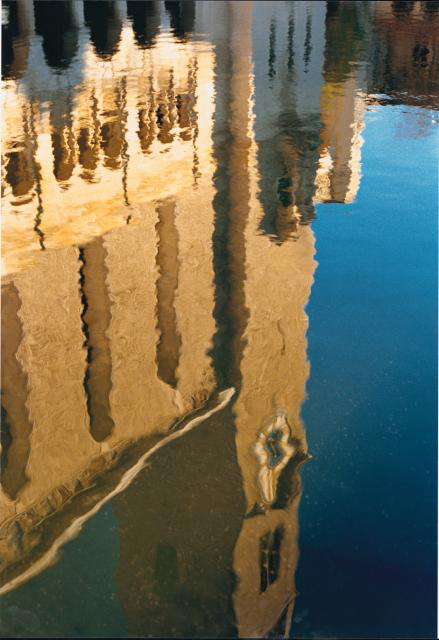
\includegraphics[height=15cm]{images/reflection.png}
\begin{table}[b]
\begin{tabular}{cccc}

\includegraphics[width=3cm]{images/UWA-Full-Hor-CMYK.png}&

\includegraphics[width=3cm]{images/PCB.png}&
School of Psychological Science &
Institute of Advanced Studies
\end{tabular}
\end{table}
\end{center}

\pagebreak

\section{Welcome}\label{welcome}

We are delighted to welcome you to the 2018 Australian Mathematical
Psychology Conference in Perth, Western Australia. We look forward a day
of workshops on important topics and methods in mathematical psychology
(13th February), a public lecture by Prof Amy Criss on her work (13th
February) and two days of talks lying in the intersection
\(Maths \cap Psychology\) (14-15 February).

We gratefully acknowledge the support of the Office of the Deputy
Vice-Chancellor (Research) at UWA, the Institute of Advanced Studies
(UWA), the UWA School of Psychological Science, and the Perth Convention
Bureau. We would also like to thank those contributing to workshops,
especially Prof Amy Criss, who will be leading one of the workshops as
well as giving a public lecture on her work.

\vspace{0.5cm}

Simon Farrell, Alice Mason, John Dunn, Ullrich Ecker, and Mark Hurlstone
Organising Committee

\vspace{1cm}

\emph{The University of Western Australia acknowledges that it is
situated on Noongar land, that the Noongar people remain the spiritual
and cultural custodians of their land and continue to practise their
values, languages, beliefs and knowledge.}

\pagebreak

\section{Venue}\label{venue}

The workshops and conference talks will be held in the Conference Room,
St Catherine's College. St Catherine's College is located just north of
the UWA campus. Tea and coffee will be provided, along with snacks in
the morning and afternoon. Cafes for lunch are located on the main
campus (Hackett Cafe, Village Cafe, Reid Library) as well as on Hampden
Road.

\begin{center}
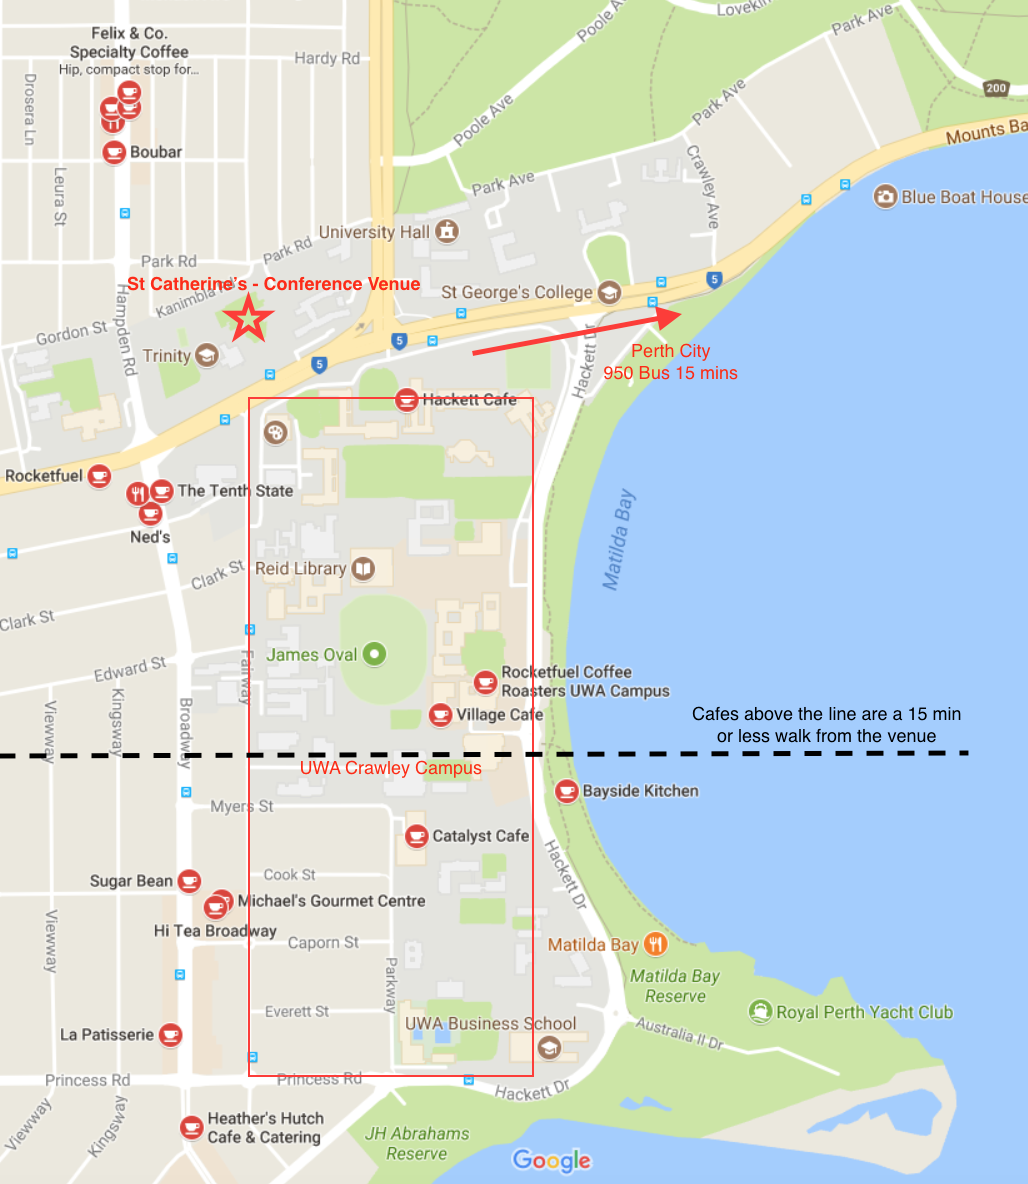
\includegraphics[width=16cm]{images/Venue.png}
\end{center}

\section{Soccer}\label{soccer}

Following the talks on 14th February, we will proceed to Riley Oval (map
below) for some soccer action. For those who prefer not to play, there
are some pleasant places nearby to sit and talk.

\begin{center}

\includegraphics[width=10cm]{images/Soccer.png}
\end{center}

\section{Conference dinner}\label{conference-dinner}

The conference dinner will be held at Jojo's from 6pm on 15th February
(last day of talks). Dinners are usually held during the conference, but
the flight schedules mean that most people will be flying out on 16th
anyway, and this means no-one needs to worry about drinking before a 9am
talk the next day.

Drinks will be from 6pm, and we will be seated for dinner around 7.

\begin{center}

\includegraphics[width=10cm]{images/Dinner.png}
\end{center}

\section{Other Activities}\label{other-activities}

\href{http://perthtouristcentre.com.au}{Perth Tourist Centre} has links
to a variety of activities in the Perth area. Typical destinations are:

\begin{itemize}
\tightlist
\item
  The Perth International Arts Festival runs from early Feb, with a good
  variety of plays, music, visual arts, and other happenings.
  \url{https://www.perthfestival.com.au/whats-on}
\item
  Beach! Cottesloe Beach is popular, and can be reached by bus or train
  (and a 10 min walk).
\item
  Swan Valley (30--45 mins outside Perth) hosts a number of wineries and
  breweries that do decent food.
  \url{https://www.swanvalley.com.au/Home}
\item
  Fremantle (coffee, shopping, old buildings)
\item
  Rottnest Island. Picturesque, with lovely beaches and a great place to
  go cycling. Ferries depart from Fremantle; you'll want to make it a
  day trip.
\item
  Shopping: Perth CBD and Claremont Quarter are nearby (10--15 mins by
  bus).
\item
  Relax: If you want to chill out and relax, Matilda Bay and Kings Park
  are both nearby and offer nice scenery. Kings Park also has some good
  walking and running tracks.
\item
  Cruises: There are a variety of cruises around Fremantle and on the
  Swan. See over for a discount with Captain Cook Cruises.
\end{itemize}

{[}Alice, could you put some stuff here about eating out and drinking.
Places nearby (e.g., Varsity) and in the city{]}

\begin{center}

\includegraphics[width=10cm]{images/CCC.pdf}
\end{center}

\pagebreak

\section{Tuesday 2018-02-13}\label{tuesday-2018-02-13}

\subsection{Morning: Workshop A: Professional Development
Symposium}\label{morning-workshop-a-professional-development-symposium}

Panel Discussion on Gender and STEM - St Catherine's college 10 am-12
noon

This career development workshop aims to promote gender equality and
diversity in mathematical psychology. Follow this link to read more
about the workshop and register:
\url{http://www.ias.uwa.edu.au/masterclass/STEMresearch}.

Professor Amy Criss will be joined in a panel discussion by Associate
Professor Amy Perfors (University of Melbourne) and Associate Professor
Chris Donkin (UNSW). Discussion will be facilitated by Dr Alice Mason
(UWA) who is chair of the Gender Diversity Committee in the School of
Psychological Science. This masterclass is open to attendees of any
gender.

Prof Criss is Head of Discipline (Psychology) at Syracuse, a
world-leading expert in the computational modelling of human memory.
Prof Criss has been
\href{http://memolab.syr.edu/Pride.html}{substantially involved} in
efforts to enhance diversity in undergraduate students, and was
President of the Society for Mathematical Psychology. Prof Criss
involvement is supported by UWA's Institute of Advanced Studies.

If you have any questions please contact Alice Mason
(\href{mailto:alice.mason@uwa.edu.au}{\nolinkurl{alice.mason@uwa.edu.au}}).

\subsection{Afternoon: Workshop B: State-trace
Analysis}\label{afternoon-workshop-b-state-trace-analysis}

Presenters: John Dunn, Mike Kalish, Rachel Stephens St Catherine's
college 2pm--5pm

The aim of this workshop is to provide a brief introduction to the
application of state-trace analysis (STA) to psychological data based on
the book

Dunn, J.C. \& Kalish, M. L. (in press). \emph{State-trace analysis}.
Springer.

The following aspects will be covered (time permitting):

\begin{enumerate}
\def\labelenumi{\arabic{enumi}.}
\item
\begin{verbatim}
 Brief introduction to the logic of STA
\end{verbatim}
\item
\begin{verbatim}
 Fitting the monotonic model
\end{verbatim}
\item
\begin{verbatim}
 Analysis of continuous data
\end{verbatim}
\item
\begin{verbatim}
 Analysis of discrete data
\end{verbatim}
\end{enumerate}

Those attending will need to bring their own laptop to take part in the
activities. Some software will need to be installed prior to the
workshop; details can be found at
\url{https://alicemason.github.io/AMPC18/_pages/Workshops/}

\subsection{Evening: Public lecture by Prof Amy
Criss}\label{evening-public-lecture-by-prof-amy-criss}

Professor Amy Criss will be giving an Institute of Advanced Studies
public lecture 6pm--7pm on the 13th in Woolnough Lecture Theatre,
Geology Building, UWA (a 5--10 min walk from St Catherines). The talk is
titled ``How remembering causes forgetting''. You can find out more
details and book a seat: \url{http://www.ias.uwa.edu.au/lectures/criss}

``Humans rely on memory at nearly every moment: we use our memories of
the past to predict the future, and memory is essential to our concept
of self. Nevertheless, our memory for the details of events is
imperfect. Some details of an event are forgotten and other details can
be falsely remembered. One other striking characteristic of memory is
that that act of remembering can change what is being remembered:
retrieving events from memory changes our memory of those individual
events.

``In this talk Professor Amy Criss will explain how the effects of
retrieval on memory can be understood using carefully designed
experiments, and show that the accuracy of memory for an event declines
as we repeatedly recall that event. She will also discuss how theories
of memory can be expressed as computational models, and how we can use
computational models to understand how forgetting is caused by
remembering.''

\pagebreak  

\section{Wednesday 2018-02-14}\label{wednesday-2018-02-14}

\subsection{Morning}\label{morning}

\begin{longtable}[]{@{}lll@{}}
\toprule
\begin{minipage}[b]{0.03\columnwidth}\raggedright\strut
Time\strut
\end{minipage} & \begin{minipage}[b]{0.38\columnwidth}\raggedright\strut
Authors\strut
\end{minipage} & \begin{minipage}[b]{0.51\columnwidth}\raggedright\strut
Title\strut
\end{minipage}\tabularnewline
\midrule
\endhead
\begin{minipage}[t]{0.03\columnwidth}\raggedright\strut
09:00\strut
\end{minipage} & \begin{minipage}[t]{0.38\columnwidth}\raggedright\strut
\strut
\end{minipage} & \begin{minipage}[t]{0.51\columnwidth}\raggedright\strut
Welcome\strut
\end{minipage}\tabularnewline
\begin{minipage}[t]{0.03\columnwidth}\raggedright\strut
09:10\strut
\end{minipage} & \begin{minipage}[t]{0.38\columnwidth}\raggedright\strut
\textbf{Amy Perfors}, Nicholas van Dam\strut
\end{minipage} & \begin{minipage}[t]{0.51\columnwidth}\raggedright\strut
Decision-making in black swan environments\strut
\end{minipage}\tabularnewline
\begin{minipage}[t]{0.03\columnwidth}\raggedright\strut
09:30\strut
\end{minipage} & \begin{minipage}[t]{0.38\columnwidth}\raggedright\strut
\textbf{John C. Dunn} , Li-Lin Rao\strut
\end{minipage} & \begin{minipage}[t]{0.51\columnwidth}\raggedright\strut
Models of risky choice: A signed difference analysis\strut
\end{minipage}\tabularnewline
\begin{minipage}[t]{0.03\columnwidth}\raggedright\strut
09:50\strut
\end{minipage} & \begin{minipage}[t]{0.38\columnwidth}\raggedright\strut
\textbf{Christina Van Heer}, Robert Hester, David K. Sewell, Philip L.
Smith\strut
\end{minipage} & \begin{minipage}[t]{0.51\columnwidth}\raggedright\strut
The role of prediction error and confidence in sequential
decisions\strut
\end{minipage}\tabularnewline
\begin{minipage}[t]{0.03\columnwidth}\raggedright\strut
10:00\strut
\end{minipage} & \begin{minipage}[t]{0.38\columnwidth}\raggedright\strut
\textbf{Jared M. Hotaling}, Andreas Jarvstad, Chris Donkin, Ben R.
Newell\strut
\end{minipage} & \begin{minipage}[t]{0.51\columnwidth}\raggedright\strut
The effects of outcome information during sampling on decisions from
experience\strut
\end{minipage}\tabularnewline
\begin{minipage}[t]{0.03\columnwidth}\raggedright\strut
10:20\strut
\end{minipage} & \begin{minipage}[t]{0.38\columnwidth}\raggedright\strut
\textbf{Yiyun Shou} , Michael Smithson\strut
\end{minipage} & \begin{minipage}[t]{0.51\columnwidth}\raggedright\strut
How Do People Think About the Probability of Human Extinction?\strut
\end{minipage}\tabularnewline
\begin{minipage}[t]{0.03\columnwidth}\raggedright\strut
10:40\strut
\end{minipage} & \begin{minipage}[t]{0.38\columnwidth}\raggedright\strut
\strut
\end{minipage} & \begin{minipage}[t]{0.51\columnwidth}\raggedright\strut
\textbf{Coffee}\strut
\end{minipage}\tabularnewline
\begin{minipage}[t]{0.03\columnwidth}\raggedright\strut
11:10\strut
\end{minipage} & \begin{minipage}[t]{0.38\columnwidth}\raggedright\strut
\textbf{Ashley Luckman}, Sebastian Gluth, Jorg Rieskamp.\strut
\end{minipage} & \begin{minipage}[t]{0.51\columnwidth}\raggedright\strut
Using Response Times to distinguish between attribute-wise and
alternate-wise models of inter-temporal choice.\strut
\end{minipage}\tabularnewline
\begin{minipage}[t]{0.03\columnwidth}\raggedright\strut
11:30\strut
\end{minipage} & \begin{minipage}[t]{0.38\columnwidth}\raggedright\strut
\textbf{Yonatan Vanunu}, Jared M. Hotaling, Ben R. Newell\strut
\end{minipage} & \begin{minipage}[t]{0.51\columnwidth}\raggedright\strut
The Impact of Goal and Cognitive Load on Decisions from
Experience.\strut
\end{minipage}\tabularnewline
\begin{minipage}[t]{0.03\columnwidth}\raggedright\strut
11:40\strut
\end{minipage} & \begin{minipage}[t]{0.38\columnwidth}\raggedright\strut
\textbf{Timothy Ballard}, David Sewell, Andrew Neal\strut
\end{minipage} & \begin{minipage}[t]{0.51\columnwidth}\raggedright\strut
Human information processing in the face of reward versus
punishment\strut
\end{minipage}\tabularnewline
\begin{minipage}[t]{0.03\columnwidth}\raggedright\strut
11:50\strut
\end{minipage} & \begin{minipage}[t]{0.38\columnwidth}\raggedright\strut
Rachel Mullard, Marc Adam, \textbf{Ami Eidels}\strut
\end{minipage} & \begin{minipage}[t]{0.51\columnwidth}\raggedright\strut
Competitive Decision Making in Dutch Auctions\strut
\end{minipage}\tabularnewline
\begin{minipage}[t]{0.03\columnwidth}\raggedright\strut
12:00\strut
\end{minipage} & \begin{minipage}[t]{0.38\columnwidth}\raggedright\strut
\textbf{Alice Mason}, Mark Hurlstone, Geoff Ward, Gordon Brown, Simon
Farrell\strut
\end{minipage} & \begin{minipage}[t]{0.51\columnwidth}\raggedright\strut
Evaluating bundles of numbers: assessing the trade-off between memory
and online updating in retrospective evaluation\strut
\end{minipage}\tabularnewline
\begin{minipage}[t]{0.03\columnwidth}\raggedright\strut
12:10\strut
\end{minipage} & \begin{minipage}[t]{0.38\columnwidth}\raggedright\strut
\textbf{Luke Strickland}, David Elliott, Michael David Wilson, Shayne
Loft, Andrew Heathcote\strut
\end{minipage} & \begin{minipage}[t]{0.51\columnwidth}\raggedright\strut
Modelling Prospective Memory in Simulated Maritime Surveillance:
Cognitive Control and Competition for Capacity\strut
\end{minipage}\tabularnewline
\begin{minipage}[t]{0.03\columnwidth}\raggedright\strut
12:30\strut
\end{minipage} & \begin{minipage}[t]{0.38\columnwidth}\raggedright\strut
\textbf{Russell J. Boag}, Luke Strickland, Andrew Heathcote, Shayne
Loft\strut
\end{minipage} & \begin{minipage}[t]{0.51\columnwidth}\raggedright\strut
Modelling Cognitive Control Mechanisms in Simulated Air-Traffic
Control\strut
\end{minipage}\tabularnewline
\begin{minipage}[t]{0.03\columnwidth}\raggedright\strut
12:40\strut
\end{minipage} & \begin{minipage}[t]{0.38\columnwidth}\raggedright\strut
\strut
\end{minipage} & \begin{minipage}[t]{0.51\columnwidth}\raggedright\strut
Lunch\strut
\end{minipage}\tabularnewline
\bottomrule
\end{longtable}

\subsection{Afternoon}\label{afternoon}

\begin{longtable}[]{@{}lll@{}}
\toprule
\begin{minipage}[b]{0.03\columnwidth}\raggedright\strut
Time\strut
\end{minipage} & \begin{minipage}[b]{0.39\columnwidth}\raggedright\strut
Authors\strut
\end{minipage} & \begin{minipage}[b]{0.50\columnwidth}\raggedright\strut
Title\strut
\end{minipage}\tabularnewline
\midrule
\endhead
\begin{minipage}[t]{0.03\columnwidth}\raggedright\strut
14:00\strut
\end{minipage} & \begin{minipage}[t]{0.39\columnwidth}\raggedright\strut
\textbf{Brett K. Hayes}, Rachel G. Stephens, Jeremy Ngo, John C.
Dunn\strut
\end{minipage} & \begin{minipage}[t]{0.50\columnwidth}\raggedright\strut
The dimensionality of reasoning: Inductive and deductive inference can
be explained by a single process\strut
\end{minipage}\tabularnewline
\begin{minipage}[t]{0.03\columnwidth}\raggedright\strut
14:20\strut
\end{minipage} & \begin{minipage}[t]{0.39\columnwidth}\raggedright\strut
\textbf{Dani Navarro}, Alison McCann, Alexandra Tingey, Nicole Baz,
Michelle Keshwa, Amy Perfors\strut
\end{minipage} & \begin{minipage}[t]{0.50\columnwidth}\raggedright\strut
Extensional and intensional reasoning: A Bayesian perspective on the
conjunction fallacy\strut
\end{minipage}\tabularnewline
\begin{minipage}[t]{0.03\columnwidth}\raggedright\strut
14:40\strut
\end{minipage} & \begin{minipage}[t]{0.39\columnwidth}\raggedright\strut
Mike Le Pelley, \textbf{Ben R. Newell}, Robert Nosofsky\strut
\end{minipage} & \begin{minipage}[t]{0.50\columnwidth}\raggedright\strut
Once more, with feeling: deferred feedback does not ``sharply
dissociate'' `implicit' and `explicit' category learning.\strut
\end{minipage}\tabularnewline
\begin{minipage}[t]{0.03\columnwidth}\raggedright\strut
14:50\strut
\end{minipage} & \begin{minipage}[t]{0.39\columnwidth}\raggedright\strut
\textbf{Rachel. G. Stephens}, Dora Matzke, Brett K. Hayes\strut
\end{minipage} & \begin{minipage}[t]{0.50\columnwidth}\raggedright\strut
Disappearing dissociations in experimental psychology: Using state-trace
analysis to test for multiple processes\strut
\end{minipage}\tabularnewline
\begin{minipage}[t]{0.03\columnwidth}\raggedright\strut
15:10\strut
\end{minipage} & \begin{minipage}[t]{0.39\columnwidth}\raggedright\strut
\textbf{Guillermo Campitelli}\strut
\end{minipage} & \begin{minipage}[t]{0.50\columnwidth}\raggedright\strut
The prediction game: A simple pedagogical tool to introduce Bayesian
inference\strut
\end{minipage}\tabularnewline
\begin{minipage}[t]{0.03\columnwidth}\raggedright\strut
15:30\strut
\end{minipage} & \begin{minipage}[t]{0.39\columnwidth}\raggedright\strut
\strut
\end{minipage} & \begin{minipage}[t]{0.50\columnwidth}\raggedright\strut
\textbf{Coffee}\strut
\end{minipage}\tabularnewline
\begin{minipage}[t]{0.03\columnwidth}\raggedright\strut
16:00\strut
\end{minipage} & \begin{minipage}[t]{0.39\columnwidth}\raggedright\strut
\textbf{Paul Dudgeon}, Mariska Barendse, \& Yves Rosseel\strut
\end{minipage} & \begin{minipage}[t]{0.50\columnwidth}\raggedright\strut
Leverage-based confidence intervals for structural equation
modelling.\strut
\end{minipage}\tabularnewline
\begin{minipage}[t]{0.03\columnwidth}\raggedright\strut
16:20\strut
\end{minipage} & \begin{minipage}[t]{0.39\columnwidth}\raggedright\strut
\textbf{Nicolas Fay} , Bradley Walker\strut
\end{minipage} & \begin{minipage}[t]{0.50\columnwidth}\raggedright\strut
Applying the Cultural Ratchet to a Social Artefact: The Cumulative
Cultural Evolution of a Language Game\strut
\end{minipage}\tabularnewline
\begin{minipage}[t]{0.03\columnwidth}\raggedright\strut
16:40\strut
\end{minipage} & \begin{minipage}[t]{0.39\columnwidth}\raggedright\strut
\textbf{Bradley Walker}, Nicolas Fay\strut
\end{minipage} & \begin{minipage}[t]{0.50\columnwidth}\raggedright\strut
An Egocentric Bias is Important to Adaptive Social Learning\strut
\end{minipage}\tabularnewline
\begin{minipage}[t]{0.03\columnwidth}\raggedright\strut
16:50\strut
\end{minipage} & \begin{minipage}[t]{0.39\columnwidth}\raggedright\strut
\textbf{Matthew B. Thompson}, Rachel A. Searston, Gianni Ribeiro, Jason
M. Tangen\strut
\end{minipage} & \begin{minipage}[t]{0.50\columnwidth}\raggedright\strut
Alternative statistical frameworks for communicating the strength of
forensic evidence in court\strut
\end{minipage}\tabularnewline
\begin{minipage}[t]{0.03\columnwidth}\raggedright\strut
17:10\strut
\end{minipage} & \begin{minipage}[t]{0.39\columnwidth}\raggedright\strut
\textbf{Matthew Kaesler}, John Dunn, Carolyn Semmler\strut
\end{minipage} & \begin{minipage}[t]{0.50\columnwidth}\raggedright\strut
Evaluating Signal Detection Models for Eyewitness Identification\strut
\end{minipage}\tabularnewline
\begin{minipage}[t]{0.03\columnwidth}\raggedright\strut
17:20\strut
\end{minipage} & \begin{minipage}[t]{0.39\columnwidth}\raggedright\strut
\textbf{Simon De Deyne} , Amy Perfors\strut
\end{minipage} & \begin{minipage}[t]{0.50\columnwidth}\raggedright\strut
Near neighbour judgements as an efficient way to estimate semantic
similarity.\strut
\end{minipage}\tabularnewline
\begin{minipage}[t]{0.03\columnwidth}\raggedright\strut
17:30\strut
\end{minipage} & \begin{minipage}[t]{0.39\columnwidth}\raggedright\strut
\strut
\end{minipage} & \begin{minipage}[t]{0.50\columnwidth}\raggedright\strut
Soccer\strut
\end{minipage}\tabularnewline
\bottomrule
\end{longtable}

\pagebreak  

\section{Thursday 2018-02-15}\label{thursday-2018-02-15}

\subsection{Morning}\label{morning-1}

\begin{longtable}[]{@{}lll@{}}
\toprule
\begin{minipage}[b]{0.03\columnwidth}\raggedright\strut
Time\strut
\end{minipage} & \begin{minipage}[b]{0.35\columnwidth}\raggedright\strut
Authors\strut
\end{minipage} & \begin{minipage}[b]{0.53\columnwidth}\raggedright\strut
Title\strut
\end{minipage}\tabularnewline
\midrule
\endhead
\begin{minipage}[t]{0.03\columnwidth}\raggedright\strut
09:00\strut
\end{minipage} & \begin{minipage}[t]{0.35\columnwidth}\raggedright\strut
\textbf{Chi-Fai Lo}, Kwok-Kwan Wong and Ho-Yan Ip\strut
\end{minipage} & \begin{minipage}[t]{0.53\columnwidth}\raggedright\strut
Lie-algebraic Approach for the Leaky Competing Accumulator Model of
Decision Making\strut
\end{minipage}\tabularnewline
\begin{minipage}[t]{0.03\columnwidth}\raggedright\strut
09:20\strut
\end{minipage} & \begin{minipage}[t]{0.35\columnwidth}\raggedright\strut
Yakov Ben-Haim, \textbf{Michael Smithson}\strut
\end{minipage} & \begin{minipage}[t]{0.53\columnwidth}\raggedright\strut
Assessing Robustness of Statistical Models: Info-Gap Theory\strut
\end{minipage}\tabularnewline
\begin{minipage}[t]{0.03\columnwidth}\raggedright\strut
09:40\strut
\end{minipage} & \begin{minipage}[t]{0.35\columnwidth}\raggedright\strut
\textbf{Don van Ravenzwaai}, Casper Albers, Henk Kiers\strut
\end{minipage} & \begin{minipage}[t]{0.53\columnwidth}\raggedright\strut
Credible Confidence: A pragmatic view on the frequentist vs Bayesian
debate\strut
\end{minipage}\tabularnewline
\begin{minipage}[t]{0.03\columnwidth}\raggedright\strut
10:00\strut
\end{minipage} & \begin{minipage}[t]{0.35\columnwidth}\raggedright\strut
\textbf{Trisha Nowland}\strut
\end{minipage} & \begin{minipage}[t]{0.53\columnwidth}\raggedright\strut
Mathematical Set Theory for Latent Variable Modelling in Psychology
Research\strut
\end{minipage}\tabularnewline
\begin{minipage}[t]{0.03\columnwidth}\raggedright\strut
10:10\strut
\end{minipage} & \begin{minipage}[t]{0.35\columnwidth}\raggedright\strut
\textbf{Daniel Feuerriegel}, Daniel Bennett, Phillip M. Alday, Stefan
Bode\strut
\end{minipage} & \begin{minipage}[t]{0.53\columnwidth}\raggedright\strut
The Decision Decoding Toolbox (DDTBOX) - A multivariate pattern analysis
toolbox for event-related potentials\strut
\end{minipage}\tabularnewline
\begin{minipage}[t]{0.03\columnwidth}\raggedright\strut
10:30\strut
\end{minipage} & \begin{minipage}[t]{0.35\columnwidth}\raggedright\strut
\strut
\end{minipage} & \begin{minipage}[t]{0.53\columnwidth}\raggedright\strut
\textbf{Coffee}\strut
\end{minipage}\tabularnewline
\begin{minipage}[t]{0.03\columnwidth}\raggedright\strut
11:00\strut
\end{minipage} & \begin{minipage}[t]{0.35\columnwidth}\raggedright\strut
\textbf{Klaus Oberauer}, Hsuan-Yu Lin\strut
\end{minipage} & \begin{minipage}[t]{0.53\columnwidth}\raggedright\strut
An Interference Model of Visual Working Memory: Applications to Change
Detection\strut
\end{minipage}\tabularnewline
\begin{minipage}[t]{0.03\columnwidth}\raggedright\strut
11:20\strut
\end{minipage} & \begin{minipage}[t]{0.35\columnwidth}\raggedright\strut
Anthea G. Blunden, Dylan Hammond, Piers D. L. Howe, \textbf{Daniel R.
Little}\strut
\end{minipage} & \begin{minipage}[t]{0.53\columnwidth}\raggedright\strut
Characterising the architecture and integration rule of change detection
decisions\strut
\end{minipage}\tabularnewline
\begin{minipage}[t]{0.03\columnwidth}\raggedright\strut
11:40\strut
\end{minipage} & \begin{minipage}[t]{0.35\columnwidth}\raggedright\strut
\textbf{Chris Donkin}\strut
\end{minipage} & \begin{minipage}[t]{0.53\columnwidth}\raggedright\strut
Inferring task-specific psychological representation\strut
\end{minipage}\tabularnewline
\begin{minipage}[t]{0.03\columnwidth}\raggedright\strut
11:50\strut
\end{minipage} & \begin{minipage}[t]{0.35\columnwidth}\raggedright\strut
\textbf{Marton Kocsis}, Simon Farrell\strut
\end{minipage} & \begin{minipage}[t]{0.53\columnwidth}\raggedright\strut
The Role of Working Memory in Free Recall: The Effect of Preload at
Retrieval\strut
\end{minipage}\tabularnewline
\begin{minipage}[t]{0.03\columnwidth}\raggedright\strut
12:00\strut
\end{minipage} & \begin{minipage}[t]{0.35\columnwidth}\raggedright\strut
\textbf{Adam F. Osth} , Simon Farrell\strut
\end{minipage} & \begin{minipage}[t]{0.53\columnwidth}\raggedright\strut
Modeling response time distributions of free recall initiation with race
models\strut
\end{minipage}\tabularnewline
\begin{minipage}[t]{0.03\columnwidth}\raggedright\strut
12:20\strut
\end{minipage} & \begin{minipage}[t]{0.35\columnwidth}\raggedright\strut
\textbf{Kevin D. Shabahang}, D. J. K. Mewhort, Donald R. J.
Franklin,\strut
\end{minipage} & \begin{minipage}[t]{0.53\columnwidth}\raggedright\strut
Semantic contrast effects: a holographic interface linking episodic and
semantic memory\strut
\end{minipage}\tabularnewline
\begin{minipage}[t]{0.03\columnwidth}\raggedright\strut
12:30\strut
\end{minipage} & \begin{minipage}[t]{0.35\columnwidth}\raggedright\strut
\strut
\end{minipage} & \begin{minipage}[t]{0.53\columnwidth}\raggedright\strut
Lunch\strut
\end{minipage}\tabularnewline
\bottomrule
\end{longtable}

\subsection{Afternoon}\label{afternoon-1}

\begin{longtable}[]{@{}lll@{}}
\toprule
\begin{minipage}[b]{0.03\columnwidth}\raggedright\strut
Time\strut
\end{minipage} & \begin{minipage}[b]{0.32\columnwidth}\raggedright\strut
Authors\strut
\end{minipage} & \begin{minipage}[b]{0.57\columnwidth}\raggedright\strut
Title\strut
\end{minipage}\tabularnewline
\midrule
\endhead
\begin{minipage}[t]{0.03\columnwidth}\raggedright\strut
13:50\strut
\end{minipage} & \begin{minipage}[t]{0.32\columnwidth}\raggedright\strut
\textbf{Roger Ratcliff}\strut
\end{minipage} & \begin{minipage}[t]{0.57\columnwidth}\raggedright\strut
Modeling Numeracy Decisions on a Continuous Scale\strut
\end{minipage}\tabularnewline
\begin{minipage}[t]{0.03\columnwidth}\raggedright\strut
14:10\strut
\end{minipage} & \begin{minipage}[t]{0.32\columnwidth}\raggedright\strut
\textbf{Philip L. Smith}, Elaine A. Corbett\strut
\end{minipage} & \begin{minipage}[t]{0.57\columnwidth}\raggedright\strut
Modelling Speeded Multielement Decision Making as Diffusion in a
Hypersphere\strut
\end{minipage}\tabularnewline
\begin{minipage}[t]{0.03\columnwidth}\raggedright\strut
14:30\strut
\end{minipage} & \begin{minipage}[t]{0.32\columnwidth}\raggedright\strut
\textbf{Guy E. Hawkins}, Nathan J. Evans, Scott D. Brown\strut
\end{minipage} & \begin{minipage}[t]{0.57\columnwidth}\raggedright\strut
Normative theories are nice, but people aren't always normative:
Comparing collapsing and fixed threshold models of speeded decision
making\strut
\end{minipage}\tabularnewline
\begin{minipage}[t]{0.03\columnwidth}\raggedright\strut
14:50\strut
\end{minipage} & \begin{minipage}[t]{0.32\columnwidth}\raggedright\strut
\textbf{Andrew Heathcote}, Mathieu Servant, Kirsty Hannah, Dora
Matzke\strut
\end{minipage} & \begin{minipage}[t]{0.57\columnwidth}\raggedright\strut
Priming and Variable Control in Choice Conflict Tasks\strut
\end{minipage}\tabularnewline
\begin{minipage}[t]{0.03\columnwidth}\raggedright\strut
15:10\strut
\end{minipage} & \begin{minipage}[t]{0.32\columnwidth}\raggedright\strut
\textbf{Quentin F. Gronau}, Andrew Heathcote, Dora Matzke\strut
\end{minipage} & \begin{minipage}[t]{0.57\columnwidth}\raggedright\strut
Warp-III Bridge Sampling for Comparing LBA Models\strut
\end{minipage}\tabularnewline
\begin{minipage}[t]{0.03\columnwidth}\raggedright\strut
15:20\strut
\end{minipage} & \begin{minipage}[t]{0.32\columnwidth}\raggedright\strut
\strut
\end{minipage} & \begin{minipage}[t]{0.57\columnwidth}\raggedright\strut
\textbf{Coffee}\strut
\end{minipage}\tabularnewline
\begin{minipage}[t]{0.03\columnwidth}\raggedright\strut
15:50\strut
\end{minipage} & \begin{minipage}[t]{0.32\columnwidth}\raggedright\strut
\textbf{Simon Dennis}, Paul Garrett, Hyungwook Yim, Nathan Evans, Vishnu
Sreekumar\strut
\end{minipage} & \begin{minipage}[t]{0.57\columnwidth}\raggedright\strut
Predicting memory for WHEN\strut
\end{minipage}\tabularnewline
\begin{minipage}[t]{0.03\columnwidth}\raggedright\strut
16:10\strut
\end{minipage} & \begin{minipage}[t]{0.32\columnwidth}\raggedright\strut
\textbf{Julian Fox}, Adam Osth \& Simon Dennis\strut
\end{minipage} & \begin{minipage}[t]{0.57\columnwidth}\raggedright\strut
Modelling condition order effects: Interference, learning, and decision
strategies\strut
\end{minipage}\tabularnewline
\begin{minipage}[t]{0.03\columnwidth}\raggedright\strut
16:20\strut
\end{minipage} & \begin{minipage}[t]{0.32\columnwidth}\raggedright\strut
\textbf{Amy H. Criss}, Jack Wilson\strut
\end{minipage} & \begin{minipage}[t]{0.57\columnwidth}\raggedright\strut
Output Interference and Release in Cued Recall: The role of learning
during test and a response filter\strut
\end{minipage}\tabularnewline
\begin{minipage}[t]{0.03\columnwidth}\raggedright\strut
16:40\strut
\end{minipage} & \begin{minipage}[t]{0.32\columnwidth}\raggedright\strut
\textbf{Christopher R. Brydges}, Gilles E. Gignac, Ullrich K. H.
Ecker\strut
\end{minipage} & \begin{minipage}[t]{0.57\columnwidth}\raggedright\strut
Working memory capacity predicts ongoing reliance on misinformation: A
latent-variable analysis\strut
\end{minipage}\tabularnewline
\begin{minipage}[t]{0.03\columnwidth}\raggedright\strut
16:50\strut
\end{minipage} & \begin{minipage}[t]{0.32\columnwidth}\raggedright\strut
\textbf{Hyungwook Yim}, Adam F. Osth, Vladimir M. Sloutsky, Simon J.
Dennis\strut
\end{minipage} & \begin{minipage}[t]{0.57\columnwidth}\raggedright\strut
Decomposing Different Sources of Interference in Recognition Memory
Development - a Computational Modeling Approach\strut
\end{minipage}\tabularnewline
\begin{minipage}[t]{0.03\columnwidth}\raggedright\strut
17:10\strut
\end{minipage} & \begin{minipage}[t]{0.32\columnwidth}\raggedright\strut
\textbf{Jason Zhou}, Philip Smith, Adam Osth, Simon Lilburn\strut
\end{minipage} & \begin{minipage}[t]{0.57\columnwidth}\raggedright\strut
Decision-Making in Source Memory: Re-evaluating the Thresholded Nature
of Source Memory Retrieval\strut
\end{minipage}\tabularnewline
\begin{minipage}[t]{0.03\columnwidth}\raggedright\strut
17:20\strut
\end{minipage} & \begin{minipage}[t]{0.32\columnwidth}\raggedright\strut
\strut
\end{minipage} & \begin{minipage}[t]{0.57\columnwidth}\raggedright\strut
Business Meeting and End of Formal Proceedings\strut
\end{minipage}\tabularnewline
\begin{minipage}[t]{0.03\columnwidth}\raggedright\strut
18:00\strut
\end{minipage} & \begin{minipage}[t]{0.32\columnwidth}\raggedright\strut
\strut
\end{minipage} & \begin{minipage}[t]{0.57\columnwidth}\raggedright\strut
Dinner\strut
\end{minipage}\tabularnewline
\bottomrule
\end{longtable}

\pagebreak

\section{Abstracts}\label{abstracts}

Timothy Ballard, David Sewell, \& Andrew Neal\\
\emph{University of Queensland}

\textbf{HUMAN INFORMATION PROCESSING IN THE FACE OF REWARD VERSUS
PUNISHMENT}

Whilst much is known about the effects of rewards and punishments on
motivation and behavior, far less is known about their effects on the
underlying information processing structures. A view held by many is
that the human information processing system has a limited capacity. The
system must therefore manage its resources efficiently, taking into
account the supply of and demand for resources when deploying them to
various tasks. According to this perspective, reward and punishment
might increase the rate of information processing, because it makes the
allocation of resources to a task a more worthwhile investment. An
alternative perspective is that the potential for reward or punishment
may slow the processing of information, because they increase the need
for resources to be deployed toward off-task activities such as
self-monitoring.

We examined these predictions using a random dot motion detection task
in which participants viewed clouds of moving dots and had to determine
whether the dots were moving mostly left or mostly right. For each
block, the participants were given the goal of being more accurate and
faster than the average participant in a pilot study. In the reward
condition, participants gained money for achieving the goal. In the
punishment condition, participants lost money for failing the goal. The
rate of information processing was measured by estimating the drift rate
parameter using the LBA model within a hierarchical Bayesian framework.

When participants were given an opportunity for reward, the average rate
of information processing did not change from baseline. However, the
amount of information required to make a decision (i.e., response
threshold) increased. When participants were under threat of punishment,
the average rate of information processing decreased, and the amount of
information required to make a decision also decreased. These findings
demonstrate the need to consider the context when attempting to
understand how information processing will unfold.\\
\pagebreak  

Yakov Ben-Haim {[}1{]} \& Michael Smithson {[}2{]}\\
\emph{{[}1{]} Technion (Israel Institute of Technology), {[}2{]} The
Australian National University}

\textbf{ASSESSING ROBUSTNESS OF STATISTICAL MODELS: INFO-GAP THEORY}

Info-gap theory provides a versatile supplement to robust statistical
techniques, by evaluating the robustness of any statistical model of a
data-set to uncertainties in any aspects of the model's functional form,
its parameters, and the data. The info-gap robustness function
quantifies the tradeoff between model accuracy and robustness. It
enables researchers to address questions such as which of several models
should be preferred for making predictions in future scenarios involving
populations that may differ in unknown ways from the data on which the
models were originally tested. We illustrate this framework with
examples using CDF-Quantile distribution models fitted to real data.\\
\pagebreak  

Anthea G. Blunden, Dylan Hammond, Piers D. L. Howe \& Daniel R. Little\\
\emph{University of Melbourne}

\textbf{CHARACTERISING THE ARCHITECTURE AND INTEGRATION OF CHANGE
DETECTION DECISIONS}

We propose an adaptation of the logical rule-based models (Fific, Little
\& Nosofsky, 2010) in order to characterise decision making based on
information held in visual short term memory. Specifically, we seek to
diagnose decision making processes in a one-shot multi-element change
detection task, as either serial, parallel, or coactive in nature. We
additionally seek to characterise whether the integration rule for each
change decision is based on the maximum evidence strength or the sum of
strengths across elements. The logical rule models assume that each
element is represented as a Gaussian distribution of perceptual effects.
To model changes, we assume that the strength of the change is
represented as a folded-normal distribution. We factorially manipulate
the magnitude of change for a given element and whether a change
decision requires an OR or an AND decision rule. This approach is novel
in that it provides a way to unify signal detection models of change
detection (Maximum Difference and Summed Difference models) with models
of information process.\\
\pagebreak  

Russell J. Boag {[}1{]}, Luke Strickland {[}2{]}, Andrew Heathcote
{[}2{]}, \& Shayne Loft {[}1{]}\\
\emph{{[}1{]} University of Western Australia, {[}2{]} University of
Tasmania}

\textbf{MODELLING COGNITIVE CONTROL MECHANISMS IN SIMULATED AIR-TRAFFIC
CONTROL}

This project uses Bayesian Linear Ballistic Accumulator (LBA) models of
decision-making to model the cognitive control mechanisms that aid
prospective memory (PM) and ongoing task performance in a complex and
dynamic air-traffic control (ATC) simulation. We aim to explain how
operators balance competing demands from ongoing and PM tasks under
different levels of time pressure, task load, and relative response
importance.

The ATC task involved classifying pairs of moving aircraft as either
`in-conflict' or `not in-conflict'. On some trials aircraft also
contained a PM target which required execution of an atypical PM
response. These decisions require the integration of multiple
information sources (e.g., relative distance, airspeed) on a dynamic
display while balancing several competing task requirements (e.g., time
pressure, PM demands, relative response importance). Moreover, decisions
typically unfolded over relatively long time-scales (up to 10 seconds).
Initial work suggests that models of simple choice such as the LBA can
account for ongoing and PM task performance in these complex, long
time-scale, less controlled applied settings.

Our modelling shows evidence of both proactive and reactive control
mechanisms. In terms of proactive control, response thresholds were
higher under PM load. This suggests individuals proactively raise
ongoing task thresholds when holding PM intentions. This effect was
larger when the importance of the PM task was emphasised and smaller
when the importance of the ongoing task was emphasised. This suggests
that holding PM intentions encourages operators to make deliberate
strategic adjustments to how they perform their primary ongoing task,
and that these adjustments vary systematically as a function of PM task
importance.\\
\pagebreak  

Christopher R. Brydges, Gilles E. Gignac, \& Ullrich K. H. Ecker\\
\emph{Universiy of Western Australia}

\textbf{WORKING MEMORY CAPACITY PREDICTS ONGOING RELIANCE ON
MISINFORMATION: A LATENT-VARIABLE ANALYSIS}

Misinformation often affects inferences and judgments even after it has
been retracted and discredited. This is known as the continued influence
effect. Memory processes have been theorized to contribute to the
continued influence effect, and much previous research has focussed on
the role of long-term memory processes at the time misinformation is
retrieved during inferential reasoning and judgments. Recently, however,
experimental research has focussed upon the role of working memory (WM)
processes engaged in the updating and integration of information, when
the retraction is encoded. From an individual differences perspective,
susceptibility to continued influence effects should be predicted by a
person's WM abilities, if continued reliance on misinformation is
influenced, at least in part, by insufficient integration of the initial
misinformation and its subsequent retraction. Consequently, we
hypothesized that WM capacity would predict susceptibility to continued
influence effects uniquely, positively, and more substantially than
short-term memory (STM) capacity. Participants (N = 216) completed a
continued-influence task, as well as a battery of WM and STM capacity
tasks. Based on a latent variable model, our hypothesis was supported
(WM capacity: beta = .36, p = .013; STM capacity: beta = -.22, p =
.187). Consequently, we suggest that WM capacity is a measurable ``risk
factor'' for continued reliance on misinformation.\\
\pagebreak  

Guillermo Campitelli\\
\emph{Edith Cowan University }

\textbf{THE PREDICTION GAME: A SIMPLE PEDAGOGICAL TOOL TO INTRODUCE
BAYESIAN INFERENCE}

In this talk I will present the prediction game, a pedagogical tool to
introduce Bayesian inference. The purpose of presenting the prediction
game is to provide a pedagogical tool to introduce Bayesian inference to
researchers or students who do not have any knowledge of Bayesian
inference. Moreover, this tool aims to solve a number of shortcomings of
introductory tutorials to Bayesian inference. (At least, all those I
examined). The main problem of introductory tutorials is that they start
too complex. They present the Bayes theorem very early on, losing most
readers in the first page. Another shortcoming is that a number of
useful components of Bayesian inference are missing. For example, the
prior predictive distribution is almost never presented. The prediction
game consists of a grid with two margins: the bottom margin represents
the values of one parameter, and the right-hand side margin represents
possible values of data. By putting poker chips into the bottom margin
the player creates something equivalent to a prior probability
distribution. By sliding the poker chips through each column of the grid
the player generates a joint probability of parameter values and
possible data values. And, by adding the number of poker chips on each
row and indicating the number of poker chips in the right margin the
player develops the prior predictive distribution. When the observed
data value is announced the corresponding row is highlighted, and the
player with more chips in that row is the winner. The right margin of
that row is the marginal likelihood. The posterior distribution is
obtained by dividing all the values on that row of the grid by the
marginal likelihood. Obtaining the ratio of the marginal likelihood of
two players is the equivalent to calculating a Bayes factor.\\
\pagebreak  

Amy H. Criss \& Jack Wilson\\
\emph{Syracuse University}

\textbf{OUTPUT INTERFERENCE AND RELEASE IN CUED RECALL: THE ROLE OF
LEARNING DURING TEST AND A RESPONSE FILTER}

Output interference is the finding that performance declines with test
trial. In cued recall tasks, participants are presented with a cue word
and tasked to output the target word studied alongside. Participants may
choose to respond or not, and a response if given may be correct or
incorrect. We aim to understand the empirical pattern of output
interference in cued recall and the underlying theoretical mechanisms.
We first analyzed published cued recall data and found fewer correct and
incorrect responses across test trial. Next, we tested the contribution
of cue and target memories on output interference through a release from
output interference paradigm: one member of each pair was an exemplar
from one of two categories, and that member was either the cue word or
target word (post-cued). The critical comparison was when one category
was tested in a blocked fashion and the blocking was either by cue
category or by target category. We found that release from output
interference only occurred when the test probe included information
about the blocked words. Specifically, release occurred for blocked
cues; release occurred for blocked targets only when the test probe
included the target category, in effect treating the target category
like an extra cue. Together these data suggest that interference is
driven both by learning the test probe and by imperfect filtering of
already provided responses.\\
\pagebreak  

Simon De Deyne \& Amy Perfors\\
\emph{University of Melbourne}

\textbf{NEAR NEIGHBOUR JUDGEMENTS AS AN EFFICIENT WAY TO ESTIMATE
SEMANTIC SIMILARITY.}

A popular way to estimate how words are similar involves asking
participants to assign a magnitude judgement of similarity for a pair of
words using a rating scale. This method has various limitations
associated with the use of rating scales and lack of context when only
two items are compared. Moreover, from a practical point of view, the
procedure becomes prohibitively expensive for a large number of items.
For example, for 1,000 items, obtaining one observation per pair would
require nearly half a million judgements.

In two studies, we explore an alternative procedure in which
participants either generate or rank a small number of near neighbours
to a natural language concept. To evaluate the validity of this new
task, we used pair-wise similarities collected for 15 basic level
categories such as ``birds'' or ``tools''. For each of the categories,
we construct a sparse near neighbour graph and show that a mechanism of
spreading activation based on random walks (see De Deyne, Navarro,
Perfors \& Storms, 2016) can be used to accurately predict pair-wise
similarity judgements using a limited amount of information.

While these results suggest excellent external validity at a fraction of
the cost, we also discuss some theoretical implications about the number
of near neighbours and fundamental differences between similarity-based
and feature-based inference in natural language concepts.\\
\pagebreak  

Simon Dennis {[}1{]}, Paul Garrett {[}2{]}, Hyungwook Yim {[}1{]},
Nathan Evans {[}3{]}, \& Vishnu Sreekumar {[}4{]}\\
\emph{{[}1{]} University of Melbourne, {[}2{]} University of Newcastle,
{[}3{]} Vanderbilt University, {[}4{]} NIH Research Laboratories}

\textbf{PREDICTING MEMORY FOR WHEN}

We present a model that predicts when people will believe events from
their lives occurred on a person by person and stimulus by stimulus
basis. Participants wore a smartphone in a pouch around their necks for
two weeks. The smartphone collected timestamps, GPS, accelerometry,
audio segments and images. These data sources were augmented with
weather conditions, temperature, moon phase and tags derived from the
audio using a machine learning model. A week later they were shown a
selection of images and were required to indicate on which day each was
taken. A conditional logit model predicted leave one person out
judgements, leave one day out judgements and leave one observation out
judgements. We highlight the advantages of using cross validation over
other methods of model selection.\\
\pagebreak  

Chris Donkin\\
\emph{University of New South Wales}

\textbf{INFERRING TASK-SPECIFIC PSYCHOLOGICAL REPRESENTATION}

Most psychological theories of cognition propose that when an individual
encounters a task, they rely on a mental representation of the stimuli
used in that task. Standard approaches for measuring the mental
representation of such stimuli are explicit and subjective. For example,
observers may be asked to rate what they believe to be the similarity
between pairs of items. One of the major issues with this approach is
that one must assume that the stimuli have the same mental
representation in the similarity rating task as in any other task. Our
approach is to subvert this problem, by directly extracting the mental
representation of stimuli from the cognitive task of interest.
Specifically, we use the Generalized Context Model to infer the mental
representation of a set of 20 colors from responses in a visual working
memory task. Along the way, we also use the model to infer the strength
of memories for items on the current and previous trial, thus
investigating the role of recency, primacy, and proactive interference
in visual working memory. Finally, we also use the model to infer the
mental representation of 20 letter stimuli in a verbal working memory
task.\\
\pagebreak  

Paul Dudgeon{[}1{]}, Mariska Barendse{[}2{]}, \& Yves Rosseel{[}2{]}\\
\emph{{[}1{]} The University of Melbourne, {[}2{]} Ghent University}

\textbf{LEVERAGE-BASED CONFIDENCE INTERVALS FOR STRUCTURAL EQUATION
MODELLING.}

Leverage is a measure of how far away one individual's set of scores of
2 or more variables is from the scores of all other individuals. Besides
its usage in regression diagnostics, leverage is also used in estimators
of the covariance matrix of regression parameters when standard
assumptions of homoscedasticity and/or normality are violated---these
are called heteroscedastic-consistent (HC) estimators in the literature,
and they were originally proposed by Huber in the 1970s and by White in
the 1980s. Because linear regression is a particular form of structural
equation modelling (SEM), HC-type estimators are theoretically possible
in SEM also. However, only White's HCO estimator is currently available
in SEM. It is often referred to as a robust estimator or a sandwich
estimator in the SEM literature. This presentation develops
leverage-based sandwich estimators for deriving standard errors and
confidence intervals (CIs) in SEM. These new estimators correspond to
the HC3 estimator used in linear regression. Our research shows that the
current ``robust'' estimator used in SEM is not as robust as the
appellation given to it implies. More importantly, we show that the
incorporation of leverage into the current sandwich estimator used in
SEM results in much better coverage in CIs, even for samples sizes as
low as 50 (where current estimator's robustness bombs badly).\\
\pagebreak  

John C. Dunn {[}1{]} \& Li-Lin Rao {[}2{]}\\
\emph{{[}1{]} University of Western Australia, {[}2{]} Chinese Academy
of Sciences}

\textbf{MODELS OF RISKY CHOICE: A SIGNED DIFFERENCE ANALYSIS}

Risky choice involves selection between two or more options each of
which is a set of \emph{n} ordered pairs, (\(p_i,x_i\)) , where \(x_i\)
is a (positive, negative, or zero) payoff and \(p_i\) is its probability
of occurrence, with \(\sum_i^n p_i=1\). There are a large number of
different models of risky choice that fall into two broad classes; fixed
utility models that satisfy the condition of \emph{simple scalability}
and everything else. A prominent example of the former is Cumulative
Prospect Theory (Tversky \& Kahneman, 1992); a prominent example of the
latter is Decision Field Theory (Busemeyer \& Townsend, 1993). While it
is known that behaviour can be observed that inconsistent with all
models, this has largely been based on the construction of special
cases. We decided to test the class of fixed utility models against a
set of relatively unselected risky choices using signed difference
analysis (SDA). The advantage of this approach is that there is no
requirement to posit a particular form for the error function that links
the difference in the utility of two gambles, \emph{A} and \emph{B},
with the probability of choosing \emph{A} over \emph{B},
\(P(A \succ B)\) . We presented groups of participants with 30
\emph{variable} gambles (\emph{A}) each paired with one of four
\emph{fixed} gambles (\emph{B}) and tested the prediction of fixed
utility models that \(P(A \succ B)\) has the same order over \emph{A}
for all \emph{B} using the statistical test developed by Kalish, Dunn,
Burdakov and Sysoev (2016). We discuss the implications of the results
and explore a relatively simple extension to a (minimally) more complex
model.

\emph{References}\\
Busemeyer, J. R., \& Townsend, J. T. (1993) Decision Field Theory: A
dynamic cognition approach to decision making. \emph{Psychological
Review, 100}, 432--459.

Kalish, M. L., Dunn, J. C., Burdakov, O. P., \& Sysoev, O. (2016). A
statistical test for equality of latent orders. \emph{Journal of
Mathematical Psychology, 70}, 1-11

Tversky, A. \& Kahneman, D. (1992). Advances in prospect theory:
Cumulative representation of uncertainty. \emph{Journal of Risk and
Uncertainty, 5(4)}, 297--323.\\
\pagebreak  

Nicolas Fay \& Bradley Walker\\
\emph{The Univeristy of Western Australia}

\textbf{APPLYING THE CULTURAL RATCHET TO A SOCIAL ARTEFACT: THE
CUMULATIVE CULTURAL EVOLUTION OF A LANGUAGE GAME}

Material artefacts evolve by cumulative cultural evolution (CCE) - the
accumulation of adaptive We present a large-scale experiment
investigating the CCE of a social artefact in transmission chains, each
containing 8 adult human participants (N=408). The social artefact is
what Wittgenstein{[}Office1{]} calls a language game, the subset of
language used to perform a particular activity; in the present study,
communicating a route on a map. Two social learning conditions were
compared: Observation and Social Interaction. Participants were tasked
with accurately communicating a route on a map to the next person in the
chain. Over the experimental generations the routes were reproduced with
progressively higher accuracy in both conditions, demonstrating the CCE
of the language game. The rate of CCE was comparable across the
conditions, but route reproduction accuracy was consistently higher in
the Social Interaction condition compared to the Observation condition.
In both conditions performance improved due to the accumulation of
adaptive patterns of verbal route descriptions, and the progressive
elimination of non-adaptive patterns. Whereas the change in content was
similar across the conditions, the change in process was fundamentally
different between the Observation and Social Interaction conditions. In
conclusion, social artefacts, like material artefacts, are subject to
cumulative cultural evolution.\\
\pagebreak  

Daniel Feuerriegel {[}1{]}, Daniel Bennett {[}2,1{]}, Phillip M. Alday
{[}3{]}, \& Stefan Bode {[}1,4{]}\\
\emph{{[}1{]} University of Melbourne, {[}2{]} Princeton University,
{[}3{]} Max Planck Institute for Psycholinguistics, {[}4{]} University
of Cologne}

\textbf{THE DECISION DECODING TOOLBOX (DDTBOX) - A MULTIVARIATE PATTERN
ANALYSIS TOOLBOX FOR EVENT-RELATED POTENTIALS}

In recent years, model-based cognitive neuroscience has increasingly
used electroencephalographic (EEG) data to characterize the timing of
processes related to parameters in cognitive models. This approach has
been successfully applied based on well-known ERP components
(e.g.~Ravenzwaaij, Provost \& Brown, 2017, J. Math. Psychol.). However
subtle multivariate patterns of EEG data, revealed by multivariate
pattern analysis (MVPA), can also provide useful neural correlates of
model parameters. Here we present DDTBOX, an open-source MVPA toolbox
for EEG data. DDTBOX runs under MATLAB and is well integrated with the
EEGLAB/ERPLAB and Fieldtrip toolboxes. It trains support vector machines
(SVMs) on patterns of event-related potential (ERP) amplitude data,
following or preceding an event of interest, for classification or
regression of experimental variables. ERP amplitude patterns can be
extracted across space/electrodes (spatial decoding), time (temporal
decoding), or both (spatiotemporal decoding). DDTBOX can also extract
SVM feature weights, generate empirical chance distributions based on
permuted-labels decoding, provide estimates of the prevalence of
decodable information in the population, and perform a variety of
corrections for multiple comparisons. DDTBOX complements conventional
model-based analyses of ERP components, as subtle multivariate patterns
can be detected that would be overlooked in standard ERP component-based
analyses. These multivariate patterns can be used to predict model
parameters directly (e.g.~Grootswagers et al., 2017, J. Cogn. Neurosci.)
or to provide complementary information to inform behavioural modelling
results (e.g.~Bode et al., 2012, J. Neurosci.). In summary, DDTBOX is an
easy-to-use and open-source toolbox that allows for characterising the
time-course of information related to perceptual and cognitive
processes. It can be applied to data from a large number of experimental
paradigms and is expected to be a valuable tool for model-based
cognitive neuroscience.\\
\pagebreak  

Julian Fox, Adam Osth, \& Simon Dennis\\
\emph{University of Melbourne}

\textbf{MODELLING CONDITION ORDER EFFECTS: INTERFERENCE, LEARNING, AND
DECISION STRATEGIES}

The list length effect (LLE) -- that recognition is poorer for items
from long lists than short lists -- is a benchmark finding in memory
research. Recently, however, its existence has been debated. Dennis, Lee
and Kinnell (2008) highlighted that previously observed LLEs were due to
various confounding factors, and that when these are controlled, there
is a null LLE. This finding of a null LLE was used to argue against the
common belief that items are the primary source of interference in
recognition. Contrary to this, Brandt and colleagues demonstrated that
when analysis is restricted to the first study-test cycle in an
experiment, a LLE results; and that it's only once performance is
averaged across multiple study-test cycles that a null LLE results. They
explained that in the first study-test cycle, participants commit a
short or long list of items to memory (e.g., 20 or 80 items); but that
in the second study-test cycle, participants often study the opposite
list type, meaning that each would have committed an equal amount of
items to memory (i.e., 100 items). Their proposal was that this gradual
equating of items that participants experience throughout testing
effectively masks the LLE. The present study replicated Brandt's results
and used computational modelling to investigate the condition order
effects, particularly whether they are caused by (1) the accrual of
item-noise, (2) changes in learning or (3) changes in response
thresholds. The data was fit with variants of the Osth and Dennis (2015)
model, now extended to include the decision-making and RT components of
the drift diffusion model.\\
\pagebreak  

Quentin F. Gronau {[}1{]}, Andrew Heathcote {[}2{]}, \& Dora Matzke
{[}1{]}\\
\emph{{[}1{]} University of Amsterdam, {[}2{]} University of Tasmania}

\textbf{WARP-III BRIDGE SAMPLING FOR COMPARING LBA MODELS}

The Linear Ballistic Accumulator (LBA; Brown \& Heathcote, 2008) model
is one of the most popular choice response time models in mathematical
psychology. When fitting the LBA to experimental data,researchers are
often interested in comparing two or more possibly non-nested model
versions. The principled Bayesian solution to this problem is to compute
posterior model probabilities and Bayes factors. Both quantities rely on
the marginal likelihood of the models which is in many applications a
high-dimensional integral that usually cannot be evaluated analytically.
Here we illustrate how Warp-III bridge sampling (Meng \& Schilling,
2002) can be used to estimate the marginal likelihood for (hierarchical)
LBA models. Warp-III sampling is an advanced version of bridge sampling
that enables the efficient estimation of the marginal likelihood, even
for cases in which the posterior distribution is skewed.\\
\pagebreak  

Guy E. Hawkins {[}1{]}, Nathan J. Evans {[}2{]}, \& Scott D. Brown
{[}1{]}\\
\emph{{[}1{]} University of Newcastle, {[}2{]} Vanderbilt University}

\textbf{NORMATIVE THEORIES ARE NICE, BUT PEOPLE AREN'T ALWAYS NORMATIVE:
COMPARING COLLAPSING AND FIXED THRESHOLD MODELS OF SPEEDED DECISION
MAKING}

Theories of perceptual decision making have been dominated by the notion
of evidence accumulation to a fixed threshold; the assumption of a
process of accumulating evidence in favor of different alternatives
until some fixed threshold level is reached, which triggers a decision.
Recent theories have suggested that thresholds may not be fixed during
each decision, but rather decrease as time passes - an assumption known
as ``collapsing thresholds''. Collapsing thresholds have been proven to
lead to better performance than fixed thresholds in tasks where the
difficulty of decisions changes randomly, and in tasks where decision
speed is emphasized, for example using deadlines. Despite the
theoretical advantages of collapsing thresholds, reviews of data from
typical decision-making paradigms have supported the traditional
assumption of fixed thresholds. With data from three experiments, we
investigated whether participants adopt collapsing thresholds in those
paradigms where doing so is the optimal decision strategy. We find that
strong emphasis on decision speed - particularly the use of response
deadlines - encourages the adoption of collapsing thresholds, but this
is not the case when simply instructing people to respond speedily or
when decision difficulty varies randomly from one trial to the next. Our
results suggest that collapsing threshold models may be most useful in
deadline experiments, and this might also explain previous results
regarding the difference between humans and non-human primates on this
topic.\\
\pagebreak  

Brett K. Hayes {[}1{]}, Rachel G. Stephens {[}1{]}, Jeremy Ngo {[}1{]},
\& John C. Dunn {[}2{]}\\
\emph{{[}1{]} University of New South Wales, {[}2{]} University of
Western Australia}

\textbf{THE DIMENSIONALITY OF REASONING: INDUCTIVE AND DEDUCTIVE
INFERENCE CAN BE EXPLAINED BY A SINGLE PROCESS}

Three-experiments examined the number of latent dimensions needed to
account for inductive and deductive reasoning. In each study,
participants were presented with arguments that varied in logical
validity and consistency with background knowledge (believability), and
evaluated them according to deductive criteria (whether the conclusion
was necessarily true given the premises) or inductive criteria (whether
the conclusion was plausible given the premises). We examined factors,
which, according to dual-processing theories, modulate the contribution
of heuristic and analytic processes to reasoning: working memory load
(Experiments 1 and 2), individual working memory capacity (Experiments 1
and 2) and decision time (Experiment 3). A number of empirical
dissociations were found. Argument validity affected deduction more than
induction. Argument believability affected induction more than
deduction. Lower working memory capacity reduced sensitivity to argument
validity and increased sensitivity to argument believability, especially
under induction instructions. Reduced decision time led to decreased
sensitivity to argument validity. State-trace analyses of each
experiment, however, found that only a single underlying dimension was
required to explain patterns of inductive and deductive judgments. This
was true even when partial-order constraints were applied. This shows
that functional dissociations, which have traditionally been seen as
evidence for dual-processing accounts, are consistent with a
single-process model of reasoning.\\
\pagebreak  

Andrew Heathcote {[}1{]}, Mathieu Servant {[}2{]}, Kirsty Hannah
{[}3{]},~\& Dora Matzke {[}4{]}\\
\emph{{[}1{]} University of Tasmania,~{[}2{]} Vanderbilt
University,~{[}3{]} University of Newcastle, {[}4{]} University of
Amsterdam}

\textbf{PRIMING AND VARIABLE CONTROL~ IN~CHOICE CONFLICT TASKS}

We propose a theory of how priming caused by~choice conflict, and
variability in control deployed to resolve the conflict, affects
decision processes. We derive a measurement model with analytic
likelihoods from the theory that is able to account for the fine-grained
time course of both response speed and accuracy as quantified by delta
functions and conditional-accuracy functions. We show it provides a
unified and parametrically coherent account of behavior in the Stroop,
Simon and Flanker tasks in fits to data from two experiments each
reported by Pratte, Rouder, Morey and White, Ratcliff and Starns (2011)
as well as new data that enables conflict effects in the Simon task to
be broken into interference and facilitation components relative to a
carefully calibrated neutral condition. We then show that the theory
fails for some participants in Simon-task data collected by Forstman,
van den Wildenberg and Ridderinkhof (2008). We extend the theorie's
concept of variable control to allow complete failures to exercise any
control on some trials, causing participants to perform the wrong task,
and show the measurement model derived from the extended theory provides
a parsimonious, coherent and accurate account of data from all
participants. We end by discussing the increasing evidence for the
important role of variability in understanding cognitive control.\\
\pagebreak  

Jared M. Hotaling {[}1{]}, Andreas Jarvstad {[}2{]}, Chris Donkin
{[}1{]}, \& Ben R. Newell {[}1{]}\\
\emph{{[}1{]} University of New South Wales, {[}2{]} University of
Oxford}

\textbf{THE EFFECTS OF OUTCOME INFORMATION DURING SAMPLING ON DECISIONS
FROM EXPERIENCE}

Decisions from experience often differ from decisions based on described
alternatives. This may stem from the fact that decisions from experience
require that individuals learn about their choice alternatives by
observing potential outcomes. We investigated the roles of attention and
memory in the choice process by comparing two types of decision
procedures: a) one where monetary value information is present during
sampling, and b) one where values are revealed after sampling. In three
experiments participants made a series of choices between pairs of risky
gambles represented as urns containing different mixtures of blue and
red balls. They began each trial by sampling balls from each urn. After
observing a representative sample from each urn, participants chose
which urn they would like to draw from for a consequential payment. In
Experiment 3 some outcome samples were highlighted to increase visual
and auditory salience.

Results from all three experiments suggest that individuals place
greater weight on rare events when outcome values are absent during
sampling. This pattern is roughly consistent with the
`description-experience gap', in which decisions from description --
which likewise involve separable representations of value and
probability information -- also indicate greater weighting of rare
events relative to decisions from experience -- which do not. In
Experiment 3, we found that highlighting a rare reward increased its
salience when outcome values were present, but not when they were
absent, suggesting that highlighting rare outcome values during sampling
led participants to place greater weight on these outcomes when making
their choices. Parameter estimates from a hierarchical Bayesian prospect
theory model supported the conclusion that value-absent choices involved
greater overweighting of rare events. We discuss the implications of
these findings on our understanding of the interplay between attention,
memory, and choice.\\
\pagebreak  

Matthew Kaesler {[}1{]}, John Dunn {[}2{]}, \& Carolyn Semmler {[}1{]}\\
\emph{{[}1{]} University of Adelaide, {[}2{]} University of Western
Australia}

\textbf{EVALUATING SIGNAL DETECTION MODELS FOR EYEWITNESS
IDENTIFICATION}

Eyewitness identification researchers have only recently employed signal
detection theory (SDT) to understand witness performance on the police
lineup task, in which a witness to a crime must either select one member
from a (typically) six-person array who matches their memory of the
perpetrator, or indicate that the perpetrator is not present. In
addition to calculating empirical SDT measures from lineup data using
Receiver Operating Curve analysis, researchers have fit a model called
SDT-compound detection (SDT-CD) in attempt to discover the underlying
theoretical parameters. However, SDT-CD has been selected for use
without quantitative comparison against other potential SDT models. Of
particular relevance to model selection is the contentious proposition
that the sequential, rather than simultaneous, presentation of lineup
members leads to superior witness decision performance, as the
sequential lineup task challenges the plausibility of many SDT models
that assume simultaneous presentation of items. This work compares the
performance of three competing models; SDT-CD, a ``maximum familiarity''
model (MAX) and a novel sequential model (SDT-SEQ), in characterising
sequential lineup data by using the Parametric Bootstrap Cross-fitting
Method (PBCM). We tested both general model types (i.e.~landscaping) and
specific instances of the models as fit to 26 datasets in order to
examine issues of model mimicry. Preliminary results highlight the
challenges of using this approach to select between highly similar
models and indicate that competing models strongly mimic each other.\\
\pagebreak  

Marton Kocsis \& Simon Farrell\\
\emph{University of Western Australia}

\textbf{THE ROLE OF WORKING MEMORY IN FREE RECALL: THE EFFECT OF PRELOAD
AT RETRIEVAL}

Existing empirical evidence that suggests that working memory (WM) is
involved in free recall of information from long-term memory primarily
comes from examination of individual differences in WM capacity that ---
due to their correlational nature --- are unable to distinguish effects
at encoding from those at retrieval. In two experiments, we
experimentally manipulated WM load via an informational preload during
free recall. Participants were presented with a list of 8 words,
followed by a 4 (study 1) or 6 (study 2) digit sequence (the preload).
Participants were then asked free recall the word-list while maintaining
the digit sequence, which was then reported in serial order after free
recall of the word-list. While the preload had a small but consistent
decrement on recall accuracy across all serial positions, there was no
reliable effect on other benchmark measures of free recall. An
ex-Gaussian model was fitted to free recall response time distributions,
and it was found that preload was found to specifically affect the delay
in retrieval onset, but did not influence the rate of memory search.
Simulations of response time distributions via
random-sampling-with-replacement model of memory retrieval suggest that
preload may have influenced the recoverability of word-lists in memory.
Given previous studies has found that attention-based manipulations at
retrieval tend to impair free recall, our findings extend this research
by suggesting that attentional components of WM are more critical to
free recall than the storage capacity of WM.\\
\pagebreak  

Mike Le Pelley {[}1{]}, Ben R. Newell {[}1{]}, \& Robert Nosofsky
{[}2{]}\\
\emph{{[}1{]} University of New South Wales, {[}2{]} Indiana University}

\textbf{ONCE MORE, WITH FEELING: DEFERRED FEEDBACK DOES NOT ``SHARPLY
DISSOCIATE'' `IMPLICIT' AND `EXPLICIT' CATEGORY LEARNING.}

The controversy over multiple category-learning systems rolls on with
proponents of the multiplicity view seemingly impervious to evidence
suggesting that single system interpretations can accommodate large
tranches of the available data. In 2014, Smith et al. published
a~Psychological Science~paper in which they claimed to have found one of
the ``strongest explicit-implicit dissociations yet seen in the
categorization literature''.~In the spirit of pursuing theoretical
development, we present empirical and modelling results that appear to
categorically rule out Smith et al's key claim that deferring feedback
has a deleterious effect on tasks that require
`Information-Integration', while leaving rule-based learning intact. We
find, perhaps unsurprisingly, that delaying feedback causes a
performance decrement in tasks which require holding information about
more than one dimension in memory --~for both information-integration
AND rule-based tasks.\\
\pagebreak  

Chi-Fai Lo, Kwok-Kwan Wong, \& Ho-Yan Ip\\
\emph{The Chinese University of Hong Kong}

\textbf{LIE-ALGEBRAIC APPROACH FOR THE LEAKY COMPETING ACCUMULATOR MODEL
OF DECISION MAKING}

In this talk we have proposed a new method, namely the Lie-algebraic
approach, to tackle the Leaky Competing Accumulator (LCA) model of
decision making with multiple alternatives and time-dependent model
parameters. By exploiting the Lie symmetry of the Fokker-Planck equation
(or the Backward Kolmogorov equation) associated with the model, we have
succeeded to solve the equation and derive the joint probability density
function (p.d.f.) and marginal p.d.f. for each alternative in closed
form, subject to the natural boundary condition. With this joint p.d.f.
a likelihood function can be explicitly constructed and thus
model-fitting procedures become feasible. We have generated some time
series of the model by Monte-Carlo simulations, and applied the
maximum-likelihood analysis to examine the efficiency and accuracy of
the calibration of model parameters. The preliminary results are
satisfactory and encouraging. So far as the authors know, currently the
LCA model can be applied to cases of two or three alternatives only
because of the lack of a closed-form joint p.d.f. for the case of N
alternatives. Hence, the authors believe that the new approach will help
shed light on further studies of the LCA model.\\
\pagebreak  

Ashley Luckman, Sebastian Gluth, \& Jörg Rieskamp.\\
\emph{University of Basel}

\textbf{USING RESPONSE TIMES TO DISTINGUISH BETWEEN ATTRIBUTE-WISE AND
ALTERNATE-WISE MODELS OF INTER-TEMPORAL CHOICE.}

An important distinction in the inter-temporal choice literature is
between models which rely on attribute-wise comparisons, and those which
rely on alternate-wise comparisons. The former assume that decisions are
made by comparing attribute levels across options, i.e.~comparing the
delays involved and the amounts involved, and weighting each of these
dimensions. The later, such as discounted utility, instead assume the
decision is made by calculating a holistic value for each option
separately, then comparing these values. Recent research has found mixed
support for attribute-wise models using process tracing measures, such
as eye-tracking and mouseover designs. We suggest a new method using
response time predictions from race models of evidence accumulation to
distinguish between these two processes. Race models assume that two
streams of evidence are being accumulated. In an alternate-wise race
model we assume that each of the two accumulators is based on the value
of one of the options under consideration, while in attribute-wise race
models we assume each accumulator corresponds to one of the differences
in attributes (i.e.~delay or amount) which is being considered. These
assumptions allow the two processes to make divergent response time
predictions under simple manipulations. For instance, in a choice
between an option yielding a smaller amount of money received sooner and
an option yielding a larger amount received later, both models predict
that preference for the smaller-sooner option will increase, as its
amount increases. However, whereas an alternate-wise model will predict
a decrease in response times, because the drift rate of the
smaller-sooner option's accumulator will increase, an attribute-wise
model will predict an increase in response times, as the drift rate for
the amount difference will decrease. We present simulations confirming
these predictions, while also considering behavior under single
accumulator diffusion models and models with inhibition. Finally, we
present preliminary data from an experiment testing these predictions
against each other.\\
\pagebreak  

Alice Mason {[}1{]}, Mark Hurlstone {[}1{]}, Geoff Ward {[}2{]}, Gordon
Brown {[}3{]}, \& Simon Farrell {[}1{]}\\
\emph{{[}1{]} University of Western Australia, {[}2{]} University of
Essex, {[}3{]} University of Warwick}

\textbf{EVALUATING BUNDLES OF NUMBERS: ASSESSING THE TRADE-OFF BETWEEN
MEMORY AND ONLINE UPDATING IN RETROSPECTIVE EVALUATION}

Retrieving samples from memory is a critical tool for decision-making.
We introduce incentive compatible methods to investigate the extent to
which memory predicts evaluation. We present participants with a
sequence of monetary values and ask them to complete both a free-recall
task and a willingness to-pay (WTP) task. In order to assess whether
there is indeed a trade-off between memory-based and moment-by-moment
strategies in evaluation, we varied participants' expectation about the
upcoming task (memory or evaluation). Using Bayesian mixed effects
models, we predict WTP from both the items that were recalled and those
that were presented and discuss how the position of a value in a
sequence determines evaluation. Our findings indicate that when
participants complete both memory and evaluation tasks there is a cost
to memory accuracy, but memory is still an effective strategy for
performing evaluation.\\
\pagebreak  

Rachel Mullard, Marc Adam, \& Ami Eidels\\
\emph{University of Newcastle}

\textbf{COMPETITIVE DECISION MAKING IN DUTCH AUCTIONS}

Dutch Auction is a descending price auction where an item begins at a
set maximum price. This price is gradually lowered over a fixed amount
of time until a bidder makes a bid, at which point that bidder is
guaranteed the purchase, at the current price. Bidders must consider
(`trade-off') certainty and price: bid early and you secure the
commodity but pay a premium; bid later and the price is lower but you
risk losing the bid to another. These properties make Dutch Auction a
fascinating context for the study of competitive decision making. We
conducted a set of experiments in which triplets of participants took
part in a computerised Dutch Auction, playing against each other in
various conditions. In another experiment, the same participants played
individually against a computer opponent. I shall present our methods
and preliminary results, and discuss necessary assumptions for the
computer opponent.\\
\pagebreak  

Daniel Navarro {[}1{]}, Alison McCann {[}1{]}, Alexandra Tingey
{[}1{]},Nicole Baz {[}1{]},Michelle Keshwa {[}1{]}, \& Amy Perfors
{[}2{]},\\
\emph{{[}1{]} University of New South Wales, {[}2{]} University of
Melbourne}

\textbf{EXTENSIONAL AND INTENSIONAL REASONING: A BAYESIAN PERSPECTIVE ON
THE CONJUNCTION FALLACY}

The conjunction fallacy is one of the most striking findings in the
heuristics and biases literature, in which people rate a pair of
propositions (e.g.~Linda is a bank teller and a feminist) as more
probable than one of the constituents (e.g.~Linda is a bank teller).
This is especially likely to occur when the description of Linda is more
representative of one category (feminist) than the other. An extensive
literature on the conjunction fallacy demonstrates that the effect is
robust, but also sensitive to linguistic and pragmatic factors.

In this talk we present a Bayesian perspective on the problem. Extending
earlier work on the pragmatics of conjunction effects, we argue that
there is a degree of ambiguity to the inference problem that people need
to solve. In an extensional reasoning scenario the problem is assumed to
be to infer the properties that Linda has (in the world) and it cannot
be the case that Linda is a feminist bank teller without also being a
bank teller. In an intensional reasoning scenario the goal is to
identify the meaning of the ideas being described or communicated.
Intensional reasoning allows a conjunction to be more likely than a
constituent: if my intent is to communicate ``red circle'' to you, and
you infer ``circle'', a communication failure has occurred. In an
effective communicative system, it is necessary to be able to specify
(and to infer) the smaller of two nested sets, and conjunction
`fallacies' are necessarily permitted. Consequently, while probabilistic
reasoning models based on extensional logic do not produce conjunction
fallacies, it is entirely possible for an intensional reasoning system
to do so.

Motivated by this theoretical perspective we present a series of
experiments showing that people's behaviour in these tasks is highly
sensitive to the distinction between extensional and intensional
semantics. When a reasoning problem is framed in a way that emphasises
the communicative and social aspect to the situation, strong conjunction
effects appear. When the task is reframed to emphasise the extensional
and non-social aspects, the fallacy is either attenuated or absent. This
sensitivity occurs across many different social categories
(e.g.~feminist bank tellers) as well as reasoning about purely physical
events (dice rolls). We argue that this sensitivity to framing occurs
because people switch between solving different inference problems, both
of which are sensible but are not equivalent to each other.\\
\pagebreak  

Trisha Nowland\\
\emph{Macquaire University}

\textbf{MATHEMATICAL SET THEORY FOR LATENT VARIABLE MODELLING IN
PSYCHOLOGY RESEARCH}

The latent variable model has described as psychology's most successful
export to other fields; yet the problem of factor indeterminacy, known
to Spearman since the earliest mathematical developments in latent
variable modeling, remains unsolved. In this presentation I explore how
the historical development of set theory, which emerged in mathematics
at roughly the same time as the latent variable model in psychometrics
may support us in drawing conclusions from our research on more sturdy
ground than is otherwise truly possible with the latent variable model.
Philosophical, methodological and direct applications will be shown to
each contribute to a unifying account for the mathematical, statistical
and psychological aspects of psychometric practices which draw on latent
variable modelling techniques.\\
\pagebreak  

Klaus Oberauer \& Hsuan-Yu Lin\\
\emph{University of Zurich}

\textbf{AN INTERFERENCE MODEL OF VISUAL WORKING MEMORY: APPLICATIONS TO
CHANGE DETECTION}

Popular models of visual working memory assume that working memory is
limited by a constant resource, which is conceived as either quantized
(as in slot models) or infinitely divisible. These models share the
assumption that the probability and quality of retrieval depends on the
resource assigned to a representation in working memory. We will present
an alternative model that incorporates the principles of general
theories of memory: Retrieval is cue-based, and performance is limited
by interference arising from several sources. Representations compete
for retrieval according to the amount of activation each of them
receives at retrieval. Activation arises from three sources: Persistent
activation of representations of recently encoded items, activation from
the retrieval cue, and background noise. One item is held in the focus
of attention; this item is represented with higher precision, and
suffers less interference from competing items and from noise. So far
the model has been applied successfully to the continuous-reproduction
paradigm. Here we will apply the model to recognition/change detection;
testing how well it fares in comparison to competing models of visual
working memory.\\
\pagebreak  

Adam F. Osth {[}1{]} \& Simon Farrell {[}2{]}\\
\emph{{[}1{]} The University of Newcastle, {[}2{]} The University of
Western Australia}

\textbf{MODELING RESPONSE TIME DISTRIBUTIONS OF FREE RECALL INITIATION
WITH RACE MODELS}

Memory models have characterized retrieval in free recall as
multialternative decision making. However, the majority of these
applications have only been applied to mean response times (RTs) and not
to complete RT distributions, which offer more constraint. We fit RT
distributions of free recall initiation with both a racing diffusion
model and the linear ballistic accumulator (LBA: Brown \& Heathcote,
2008) model in a hierarchical Bayesian framework. We applied models with
various psychological assumptions about how drift rates for each serial
position are generated. Recency was either a power law or an exponential
function. Primacy was treated either as a strength boost to the early
list items so that both primacy and recency items jointly compete to be
retrieved, or as a mixture model where on some proportion of trials, the
start context is reinstated and primacy items race with little
competition from recency items. Results from a large number of datasets
strongly favor the start context reinstatement model with an exponential
recency function.\\
\pagebreak  

Amy Perfors \& Nicholas van Dam\\
\emph{University of Melbourne}

\textbf{DECISION-MAKING IN BLACK SWAN ENVIRONMENTS}

In the real world we are often faced with decisions in which the
possible outcomes are extremely good or bad but the probability of that
outcome is extremely low: winning the lottery or being struck by
lightning are prototypical examples. Should you buy a lottery ticket?
Should you climb to the top of a hill in a rainstorm? These kind of
situations are known colloquially as `Black Swan'; scenarios and create
a particularly hard decision problem. However, despite decades of
research, decision theory is relatively silent about how people do (or
should) reason about them: most of the standard tasks involve
probabilities ranging between 10\% to 90\% and the outcomes are a
manageable fraction of existing savings. In this study we evaluate how
people reason in situations when one or both options involve extremely
low probabilities (from 0.1 to 1.5\%) of very bad outcomes (losing all
of the points accumulated so far). We explore how decisions change as a
function of the number of points available and the number of `black
swan'; options available. In addition, we evaluate if people's approach
varies based on whether they are making a single bet or planning a
strategy of bets over multiple games. Finally, we present some
exploratory research investigating whether individual differences in
anxiety and tolerance of uncertainty predict differences in behaviour in
black swan situations.\\
\pagebreak  

Roger Ratcliff\\
\emph{The Ohio State University}

\textbf{MODELING NUMERACY DECISIONS ON A CONTINUOUS SCALE}

I present a model for decision making for stimuli and responses in
continuous space. The model is applied to three numeracy tasks: in one,
a two-digit number is presented and the participant has to move their
finger to a matching location on a number line, in the second, an array
of dots is presented and the participant is to move their finger to a
matching location on an arc, and in the third, an array of dots is
presented and the participant has to speak the number. The model is
composed of diffusion processes on lines and planes in which evidence
from a stimulus (distributed across space) drives the noisy decision
process which accumulates evidence over time to a criterion at which
point a response is initiated. Noise is represented as a continuous
Gaussian process. The model produces fits for the full distributions of
response times and choice probabilities across the stimulus space and
provides distributed stimulus acuity measures.\\
\pagebreak  

Kevin D. Shabahang {[}1{]}, D. J. K. Mewhort {[}2{]}, \& Donald R. J.
Franklin {[}2{]}\\
\emph{{[}1{]} University of Melbourne, {[}2{]} Queen's University}

\textbf{SEMANTIC CONTRAST EFFECTS: A HOLOGRAPHIC INTERFACE LINKING
EPISODIC AND SEMANTIC MEMORY}

Just as there are contrast effects in perception, some memories tend to
stand out in memory, with a classic example being Release from Proactive
Interference (RPI). We implemented an interface between semantic and
episodic memory as a hologram populated by subjects' lexicon (a dynamic
distributed store containing 10,000 words and their 99,990,000 pair-wise
associations). Studying a word reinforces it in the hologram and alters
the strength of all other words in proportion to their similarity to the
studied word. When studying a list of words, subjects create inter-item
associations, as a full or partial chain. Recall is prompted by a start
instruction or by the word just recalled. Momentary strength of words is
the item's simple strength plus a value contributed from a probe item's
association strength with the item. Whereas earlier implementations of
the hologram used Gaussian vectors, we added semantics to the model by
using word vectors constructed with the BEAGLE algorithm. We collected
stimuli used in a variety of RPI tasks and were able to capture
performance at the word level. Our model also captured the classic Von
Restroff isolation effect in addition to other non-semantic effects such
as the Hebb repeated list effect.\\
\pagebreak  

Yiyun Shou \& Michael Smithson\\
\emph{The Australian National University }

\textbf{HOW DO PEOPLE THINK ABOUT THE PROBABILITY OF HUMAN EXTINCTION?}

There is surprisingly little research or theory regarding how people
think about probabilities of events with extreme consequences and
unknown (but arguably very small) probabilities. Eliciting and modeling
probability judgements for such events raise both technical and
conceptual issues regarding measurement and statistics. In the present
study, participants were asked to estimate the probability of human
extinction where the cause of extinction was not specified, versus where
a specific existential threat was made salient. We report methods and
four main findings. First, people's catch-alls for extreme events were
shaped by specific examples of such events presented to them. Second,
the distributions of extinction probability judgments display a
consistent mixture of ``deniers'' and ``pessimists''. Third, these
probability estimates are associated with general optimism and anxiety.
Finally, extinction probability judgments show a strong conjunction
fallacy whereby the probability of extinction due to a specific threat
is judged to be higher than the probability of extinction generally\\
\pagebreak  

Philip L. Smith {[}1{]}, \& Elaine A. Corbett {[}1,2{]}\\
\emph{{[}1{]} University of Melbourne, {[}2{]} Trinity College, Dublin}

\textbf{MODELLING SPEEDED MULTIELEMENT DECISION MAKING AS DIFFUSION IN A
HYPERSPHERE}

We generalize the circular 2D diffusion model of Smith (2016) to provide
a new model of speeded decision-making in multielement visual displays.
We model decision making in tasks with multielement displays as evidence
accumulation by a vector-valued diffusion process in a hypersphere,
whose radius represents the decision criterion for the task. We show
that the methods used to derive response time and accuracy predictions
for the 2D model can be applied, with only minor changes, to predict
performance in higher dimensional spaces as well. We apply the model to
the double-target deficit paradigm of Duncan (1980) in which
participants judge whether briefly-presented four-element displays
contain one or two digit targets among letter distractors. A 4D version
of the hyperspherical diffusion model correctly predicted distributions
of response times and response accuracy as a function of task difficulty
in single-target and double-target versions of the task. The estimated
drift rate parameters from the model imply that the mental
representation of the decision alternatives, which we term the `decision
template' for the task, encodes both configural and local stimulus
properties. Along with its application to multielement decision making,
the model has the potential to characterize the speed and accuracy of
multiattribute decisions in studies of cognitive categorization, visual
attention, and other areas.\\
\pagebreak  

Rachel G. Stephens {[}1{]}, Dora Matzke {[}2{]}, \& Brett K. Hayes
{[}1{]}\\
\emph{{[}1{]} University of New South Wales, {[}2{]} Univeristy of
Amerstdam}

\textbf{DISAPPEARING DISSOCIATIONS IN EXPERIMENTAL PSYCHOLOGY: USING
STATE-TRACE ANALYSIS TO TEST FOR MULTIPLE PROCESSES}

Dissociations have served as a key source of evidence for theory
development in experimental psychology. Claims about the existence of
multiple distinct psychological processes or systems are often based on
demonstrations that manipulations such as working memory load, mood or
instructions have differential effects on task performance. For example,
a manipulation may have a larger effect on performance in one task, and
a smaller or no detectable effect in another, as identified by
statistical models like analysis of variance. However, inferring
distinct underlying processes based on such interaction effects can be
misleading. Such an inference depends on the strong -- and probably
often false -- assumption that underlying psychological variables map
linearly onto the observable dependent variables. Fortunately,
state-trace analysis offers an alternative approach to test for
dissociations, avoiding the linearity assumption. We apply state-trace
analysis to databases of studies from category learning and from
reasoning that have been cited as evidence for qualitatively distinct
processes. We show that many of the dissociations thought to reflect the
operation of distinct processes disappear against the stricter criteria
of state-trace analysis. We argue that it is important for experiments
to be designed with state-trace analysis in mind, and for statistical
tools to be developed so that the approach can be readily applied. This
will lead to a more rigorous foundation for theoretical claims about
distinct underlying psychological mechanisms.\\
\pagebreak  

Luke Strickland {[}1{]}, David Elliott {[}1{]}, Michael David Wilson
{[}2{]}, Shayne Loft {[}2{]}, \& Andrew Heathcote {[}1{]}\\
\emph{{[}1{]} University of Tasmania, {[}2{]} University Western
Australia}

\textbf{MODELLING PROSPECTIVE MEMORY IN SIMULATED MARITIME SURVEILLANCE:
COGNITIVE CONTROL AND COMPETITION FOR CAPACITY}

Event-Based Prospective Memory (EVPM) requires remembering to perform
intended deferred actions when particular stimuli or events are
encountered in the future. In the laboratory, the EVPM paradigm engages
participants in an ongoing task, with a requirement to make an
alternative response to occasionally presented PM target stimuli. These
paradigms typically present a simple, static stimulus on each trial,
with no time pressure to respond. We recently put forward the
`Prospective Memory Decision Control' (PMDC) model (Strickland et al.,
under review), which uses the linear ballistic accumulator (Brown \&
Heathcote, 2008) to measure possible effects of capacity sharing between
PM and ongoing tasks, proactive control over thresholds and reactive
control on PM trials. We have already fitted PMDC to basic paradigms,
and found that EVPM leads to tonic proactive control over ongoing task
decision thresholds, as well as reactive inhibition of ongoing task
processing on PM trials. We have not found capacity sharing between PM
and ongoing tasks. In the current study, we fitted PMDC to an applied
task: simulated maritime surveillance. The task required classifying
ships travelling along a display in the presence of significant time
pressure and perceptual noise. The EVPM intention required an
alternative response to ships with certain target features. Consistent
with basic PM paradigms, we found evidence of reactive inhibition of
ongoing task processing on PM trials. However, in contrast to basic
paradigms, we found capacity sharing between PM monitoring and the
ongoing task, rather than proactive control over ongoing task
thresholds. Capacity sharing likely arose in this task due to the
increased decision complexity posed by maritime surveillance. Proactive
control over ongoing task thresholds was likely not invoked due to time
pressure. Our findings exemplify how fitting a quantitative PM
architecture derived from basic tasks can provide valuable insights into
the processes that underlie PM in applied contexts.\\
\pagebreak  

Matthew B. Thompson {[}1{]}, Rachel A. Searston {[}2{]}, Gianni Ribeiro
{[}3{]}, \& Jason M. Tangen {[}3{]}\\
\emph{{[}1{]} Murdoch University, {[}2{]} The University of Melbourne,
{[}3{]} The University of Queensland}

\textbf{ALTERNATIVE STATISTICAL FRAMEWORKS FOR COMMUNICATING THE
STRENGTH OF FORENSIC EVIDENCE IN COURT}

What forensic experts should say, or should be allowed to say, about the
results of forensic comparisons has been a contentious issue in the
legal and forensic science communities. It is common practice for
forensic pattern identification experts, such as in fingerprints and
ballistics, to testify that two impressions originate from the same
source to the exclusion of all others in the absence of statistical
information. Experts have even claimed 100\% accuracy, or that the rates
of error are so improbable that they need not be considered. An
alternative framework is necessary. When, if ever, should experts claim
to have determined that two items share a common source, and should they
present error rates, or the probability of coincidental matches?

Here we explore options for the statistical representation and
communication of forensic evidence in court. We argue that we have
reached a turning point, where Australian state and federal police
jurisdictions are seeking alternative frameworks for presenting evidence
in court, but where well-considered proposals are scarce. We propose an
avenue by which the mathematical psychology community might lend their
own expertise to the problem.\\
\pagebreak  

Christina Van Heer {[}1{]}, Robert Hester {[}1{]}, David K. Sewell
{[}2{]}, \& Philip L. Smith {[}1{]}\\
\emph{{[}1{]} University of Melbourne, {[}2{]} Univeristy of Queensland}

\textbf{THE ROLE OF PREDICTION ERROR AND CONFIDENCE IN SEQUENTIAL
DECISIONS }

The mechanistic role of subjective confidence has been well
characterised in the domains of decision making and memory, but
substantially less research has investigated how confidence influences
the learning process. A representation of confidence may be useful when
learning in probabilistic environments, where outcomes or feedback are
inherently uncertain and an agent has to cope with some level of error
and, potentially, sudden changes in the environment (change points).
Previous work suggests that confidence ratings reflect the predicted
likelihood of change points and the prediction error in sequential
decisions. As such, representations of confidence may be used to track
task variables, such as change points, prediction error, and outcome
history. However, these have typically been conflated in previous work.
Thus, we sought to unpack the contributions of these in a systematic
manner. This talk will discuss preliminary findings from four empirical
studies where observers learned about outcomes sampled from a Gaussian
distribution, and made sequential predictions and confidence estimates
in their choices. The implications of these results on the mechanistic
role of confidence and prediction error in learning and decision making
will be discussed. We show that observers behaviour can be well
characterised by a simple additive learning model and that their
behaviour is remarkably consistent, over both stationary and changing
environments, and changes in paradigm.\\
\pagebreak  

Don van Ravenzwaai, Casper Albers, \& Henk Kiers\\
\emph{University of Groningen }

\textbf{CREDIBLE CONFIDENCE: A PRAGMATIC VIEW ON THE FREQUENTIST VS
BAYESIAN DEBATE}

Throughout the last few decades, a heated debate has been going on
between frequentists and Bayesians. There are substantial theoretical
and philosophical differences between both methods. Recently, a number
of papers have come out claiming that for pragmatic purposes, both
philosophies may not be all that different. In this presentation, I will
discuss work that examines numerical correspondence between frequentist
confidence intervals and Bayesian credible intervals based on
non-informative priors. I show that numerically the differences between
confidence intervals and credible intervals are very often negligible.
I'll conclude with my take on the consequences of this for the
frequentist-Bayesian debate from a practical viewpoint.\\
\pagebreak  

Yonatan~Vanunu, Jared M.~Hotaling, Ben R.~Newell\\
\emph{University of New South Wales}

\textbf{THE IMPACT OF GOAL AND COGNITIVE LOAD ON DECISIONS FROM
EXPERIENCE.}

In the past decades, numerous studies have investigated how people adapt
their decision making processes in response to cognitive demands.
However, those studies have almost exclusively considered paradigms in
which all relevant information is presented simultaneously and
conveniently to participants (i.e.~Decisions from Description), and
therefore, very little is known about how people adjust their decision
processes due to increases in cognitive demands in Decisions from
Experience.~ In order to address this issue, we suggest an adaptive
mechanism that is guided by an optimal performance-effort trade-off and
by the task's goal.~ Previous studies have shown that different tasks'
goals in experience based decisions reveal evidence for different
underlying processes. Specifically, it has been argued that extreme
values are often~overweighted~in preferential choices
(e.g.~Tsetsos~et..al, 2012), but~underweighted~in perceptual choices
(e.g.~Vandormael,~et.~al., 2017). In order to investigate this
discrepancy and the effect of cognitive load on these mechanisms, we
applied a novel paradigm in two experiments, in which the tasks' goal
was manipulated within subjects. In both versions participants were
presented with an array of numbers. In the `Preferential' task they had
to choose between a fixed reward and a gamble with an equal chance of
winning any of one of the numbers in the array. In the `Perceptual' task
the goal was to decide whether the fixed value was higher than the
average of the numbers in the array. Cognitive load was manipulated
between subjects by applying different time constraints for the array
display, and the variance of the arrays was manipulated within subjects
in order to test the impact of extreme values. Findings show that in the
`Preferential' task under high cognitive load settings, subjects tended
to pick the array more often when it had high variance (i.e.~risk
seeking), while variance had no effect in the `perceptual' task nor
under moderate cognitive load settings in either task. These findings
are consistent with the idea that extreme values influence risk
preference especially when cognitive resources are scarce.\\
\pagebreak  

Bradley Walker \& Nicholas Fay\\
\emph{University of Western Australia}

\textbf{AN EGOCENTRIC BIAS IS IMPORTANT TO ADAPTIVE SOCIAL LEARNING}

Social learning is crucial to culture and cumulative cultural evolution.
Researchers have focused on demonstrating copying behaviour and the
cognitive biases that guide it. However, people's dominant response is
to not copy the behaviour of others. Using agent-based modeling, the
present paper demonstrates that non-copying is important to adaptive
social learning. We simulated populations of agents that varied in
population size and structure. Each agent was allocated a cultural
variant from a pool of different-quality variants. At each time step
agents could copy the variant of another agent. Copying behaviour was
determined by agents' levels of content bias (preference for
high-quality variants) and coordination bias, which varied from an
egocentric bias that promoted non-copying to an alignment bias that
promoted copying. Egocentric bias maintained a larger pool of cultural
variants (compared to an alignment bias), and, consistent with Darwinian
selection dynamics, this enhanced the environment from which a content
bias could select the optimal cultural variant. This improved
population-level adaptation, especially in small populations and large
populations organized into small neighborhoods.\\
\pagebreak  

Hyungwook Yim {[}1,2{]}, Adam F. Osth {[}1{]}, Vladimir M. Sloutsky
{[}3{]}, \& Simon J. Dennis {[}1{]}\\
\emph{{[}1{]} The University of Melbourne, {[}2{]} University of
Tasmania, {[}3{]} The Ohio State University}

\textbf{DECOMPOSING DIFFERENT SOURCES OF INTERFERENCE IN RECOGNITION
MEMORY DEVELOPMENT - A COMPUTATIONAL MODELING APPROACH}

Previous studies have pointed out that there are different sources of
interference (noise) that affect recognition memory performance. For
example, it can be difficult to recognize whether I had eggs for
breakfast today if there were other items on today's breakfast menu
(these difficulties stem from item-related noise: item-noise), if I had
eggs for breakfast in the past (i.e., these difficulties stem from
context-related noise: context-noise), or if other items and other
contexts are stored in memory (i.e., background-noise). Although often
overlooked, background-noise has been shown to make the most substantial
contribution to memory performance in adults. On the other hand, there
has not been a systematic examination on how different sources of
interference change across development. Therefore, in the current study,
we examined how different sources of interference contribute to
recognition memory across development by utilizing a computational
model. The model is embedded in a hierarchical Bayesian framework and is
capable of parameterizing different sources of interference in a given
task. Preliminary data testing 4-, and 7-year-olds, and adults with a
source recognition task showed that context noise was the major factor
decreasing throughout development, whereas the change in the
contribution of item noise and background noise was minimal. The results
imply that, at least from the ages of 4 to adulthood, the major
contribution of recognition memory development stems from context
noise.\\
\pagebreak  

Jason Zhou, Philip Smith, Adam Osth, \& Simon Lilburn\\
\emph{University of Melbourne}

\textbf{DECISION-MAKING IN SOURCE MEMORY: RE-EVALUATING THE THRESHOLDED
NATURE OF SOURCE MEMORY RETRIEVAL}

Source memory is memory for the context in which items were previously
encountered. Past research has largely aimed to establish whether source
memory retrieval is better characterised as a threshold or continuous
process in two-alternative forced choice tasks, using ROC functions.
Recently, Harlow and Donaldson (2013) introduced a continuous report
paradigm to study performance in source memory tasks, and found evidence
of a retrieval threshold underlying response accuracy. However, this
account does not consider response time (RT) distributions. To
investigate the role of decision-making in source memory retrieval, this
study used the Smith (2016) circular diffusion model to introduce
diffusion analogues of the threshold and continuous models of source
memory retrieval in a replication of the Harlow and Donaldson (2013)
task. Model selection done using the BIC found support for a circular
diffusion model where memory discretely fails, as both RT and response
accuracy data suggested that there were two components in performance.\\
\pagebreak


\end{document}
